\documentclass{article}
\usepackage{amsmath, amssymb}
\usepackage{geometry}
\usepackage{actuarialsymbol}
\geometry{a4paper, margin=1in}
\usepackage{graphicx}
\usepackage{booktabs}    
\usepackage{soul}
\usepackage{enumitem}
\usepackage{hyperref}
\usepackage{listings}
\usepackage{xcolor}
\usepackage{tabularx}
\newcolumntype{Y}{>{\raggedright\arraybackslash}X}
\usepackage{pdfpages}

% SETUP LISTINGS FOR R CODE CHUNKS
\lstset{
  language        = R,            % R syntax
  basicstyle      = \ttfamily\small, % single style for everything
  keywordstyle    = \color{blue},       % override coloured keywords
  commentstyle    = \color{gray},       % override coloured comments
  stringstyle     = \color{teal},       % override coloured strings
  frame           = single,      % box around
  numbers         = none,        % no line numbers
  keepspaces      = true,        % preserve your literal spaces
  columns         = fullflexible,% let TeX typeset each line as one run
  breaklines      = false,       % no auto-wrap (avoid extra line-runs)
  showstringspaces= false        % don’t mark spaces in strings
}
\setlist{nosep}

\begin{document}

\title{Actuarial Analytics and Data notes}
\author{Charlie Galea}
\date{2025}
\maketitle

\pagebreak
\tableofcontents
\pagebreak

\section{Chapter 1}

\section{Chapter 2}


\begin{center}
    \Large{Chapter 3: Linear Regression}
\end{center}

\section{Chapter 3}

\subsection{Simple Approach to Supervised Learning}
\begin{itemize}
    \item Simple approach to supervised learning, assumes that the dependence of $Y$ on $X_1, X_2, \dots, X_p$ is linear.
    \item True regression functions are never exactly linear.
    \item Example: Sales vs TV, Radio, Newspaper.
\end{itemize}

\subsection{The Model}
\[
Y = B_0 + B_1 X + \epsilon
\]

\subsection{Least Squares Line}
\begin{itemize}
    \item Least squares line is the line that fits the data and has the smallest distance possible from the individual points to the line.
\end{itemize}

\subsection{Standard Error of Estimates}
\begin{itemize}
    \item Standard error of the slope ($B_1$) and intercept ($B_0$).
    \item There is a 95\% chance that the constructed interval will contain the true value of $B_1$.
\end{itemize}

\subsection{T Statistic}
\begin{itemize}
    \item A low p-value means that the explanatory variable (EV) has a significant effect on the response variable (RV).
    \item Overall model accuracy is assessed via this statistic.
\end{itemize}

\subsection{Multiple Linear Regression}
\[
Y = B_0 + B_1 X_1 + B_2 X_2 + \dots + B_p X_p + \epsilon
\]
\begin{itemize}
    \item \textbf{Interpreting coefficients:} A unit change in $X_j$ is associated with a $B_j$ change in $Y$, holding all other variables fixed.
    \item High correlation between predictors (multicollinearity) can complicate interpretation.
    \item In our example: Newspaper has a large p-value, indicating little effect on sales when TV and Radio are included. It may appear significant alone, but not in the full model.
\end{itemize}

\subsection{Extensions: Interactions}
\begin{itemize}
    \item Interaction between Radio and TV spending: effectiveness of TV may increase as Radio spending increases.
    \item Include an interaction term $X_{TV}\times X_{Radio}$ in the model, with its own coefficient.
    \item A low p-value for the interaction term provides evidence that $H_A: B_{int} \neq 0$.
    \item The $R^2$ often increases when a meaningful interaction is added.
\end{itemize}


\begin{lstlisting}
# Chapter 3 Lab: Linear Regression
# if needed, install these two packages

library(MASS)
library(ISLR)

# ********************************Simple Linear Regression********************************

fix(Boston)
View(Boston)
names(Boston)
lm.fit=lm(medv~lstat)
lm.fit=lm(medv~lstat,data=Boston)
attach(Boston)
lm.fit=lm(medv~lstat)
lm.fit
summary(lm.fit)
names(lm.fit)
coef(lm.fit)
# RSS (three different approaches)
deviance(lm.fit)
sum(resid(lm.fit)^2)
sum((medv - predict(lm.fit, Boston)) ^ 2) 
# Training MSE
mean((medv - predict(lm.fit, Boston)) ^ 2)
# CI for coefficients
confint(lm.fit)
# confidence interval
predict(lm.fit,data.frame(lstat=(c(5,10,15))), interval="confidence", level = 0.95)
# prediction interval
predict(lm.fit,data.frame(lstat=(c(5,10,15))), interval="prediction", level = 0.95)


plot(lstat,medv)
abline(lm.fit)
abline(lm.fit,lwd=3)
abline(lm.fit,lwd=3,col="red")
plot(lstat,medv,col="red")
plot(lstat,medv,pch=20)
plot(lstat,medv,pch="+")
plot(1:20,1:20,pch=1:20)

# dividing the plotting region into 2X2 grid of pannels
par(mfrow=c(2,2))
plot(lm.fit)
plot(predict(lm.fit), residuals(lm.fit))
plot(predict(lm.fit), rstudent(lm.fit))
plot(hatvalues(lm.fit)) #leverage statistics
which.max(hatvalues(lm.fit))

#reset the par
resetPar <- function() {
  dev.new()
  op <- par(no.readonly = TRUE)
  dev.off()
  op
}
par(resetPar())
par("mfrow")

#Or
par(mfrow=c(1,1))

# ********************************Multiple Linear Regression********************************

lm.fit=lm(medv~lstat+age,data=Boston)
summary(lm.fit)
# fit using all predictors
lm.fit=lm(medv~.,data=Boston)
summary(lm.fit)
library(car)
vif(lm.fit) # variance inflation factor
# fit using all predictors except "age"
lm.fit1=lm(medv~.-age,data=Boston)
summary(lm.fit1)
# an alternative method of excluding one predictor
lm.fit1=update(lm.fit, ~.-age)

\end{lstlisting}
\subsection{Random Theory}
\begin{itemize}
    \item Difference between confidence interval and prediction interval
    In our regression framework, we use two kinds of intervals to quantify uncertainty at a new predictor value $x_0$:

1. \textbf{Confidence Interval}
   – What it covers: the *true mean* response $f(x_0)$ (i.e.\ the average $y$ we’d see across many hypothetical samples at $x_0$).
   – Formula (simple linear regression):

   $$
     \hat y_0 \;\pm\; t_{n-2,\alpha/2}\,\mathrm{RSE}\,\sqrt{\frac{1}{n}\;+\;\frac{(x_0 - \bar X)^2}{(n-1)\,s_X^2}}
   $$

   – Interpretation: “We are 100$(1-\alpha)$% confident that this interval contains the *average* $y$ at $x_0$.”&#x20;

2. \textbf{Prediction interval (PI)}
   – What it covers: a single future observation $Y$ at $x_0$, which varies both because of uncertainty in estimating $f(x_0)$ and the irreducible noise $\epsilon$.
   – Formula (simple linear regression):

   $$
     \hat y_0 \;\pm\; t_{n-2,\alpha/2}\,\mathrm{RSE}\,\sqrt{1 \;+\;\frac{1}{n}\;+\;\frac{(x_0 - \bar X)^2}{(n-1)\,s_X^2}}
   $$

   – **Interpretation:** “We are 100$(1-\alpha)$% confident that this interval will contain *one new* $y$ at $x_0$.”&#x20;

---

### Why is the PI always wider?

Because the PI’s standard‐error term
$\sqrt{\,1 + \frac1n + \frac{(x_0 - \bar X)^2}{(n-1)\,s_X^2}\,}$
includes an extra “1” under the square‐root, reflecting the irreducible error in a single $Y$. In contrast, the CI’s term
$\sqrt{\,\frac1n + \frac{(x_0 - \bar X)^2}{(n-1)\,s_X^2}\,}$
only captures the uncertainty in estimating the *mean* at $x_0$.&#x20;

---

In practice

* Use R’s built‐in `predict()` on an `lm` object with `interval="confidence"` or `interval="prediction"`.
* Remember: **CI** → average response; **PI** → individual response.

\end{itemize}
\pagebreak


\begin{center}
    \Large{Chapter 4: Classification}
\end{center}
\section{Chapter 4}

\subsection{4.1 Introduction to classification problems}

\begin{itemize}
    \item Looking at when the response variable has 2 or more values.
    \item The task of the classification is to build a function $C(X)$ s.t. it take the feature vector $X$ and predicts its value for $Y$
    \item Can linear regression be used?
    \begin{itemize}
        \item Yes. Make an indicator (0 if no, 1 if yes) and perform simple linear regression. $\hat{Y}>0.5$
        \item However linear regression may produce probabilities less than zero or bigger than one.
        \item If there are 3 levels, (1,2,3) linear regression is not appropriate.
    \end{itemize}
    \item Logistic regression is more appropriate.
\end{itemize}


\subsection{Logistic regression}
\begin{itemize}
    \item Lets say $p(X) = Pr(Y = 1|X)$ for sure and consider using balance to predict default. Logistic regression uses the form,
    \begin{equation*}
        p(X) = \frac{e^{\beta_0 + \beta_1 X}}{1 + e^{\beta_0 + \beta_1 X}}
    \end{equation*}
    \item since we can transform it to
    \begin{equation*}
        \log(\frac{p(X)}{1 - p(X)}) = \beta_0 + \beta_1 X
    \end{equation*}
    \item We can use maximum likelihood to estimate the regression coefficients.
    \begin{equation*}
        \ell(\beta_0,\beta) = \prod_{i:y_i=1} p(x_i) \; \prod_{i:y_i} (1 - p(x_i))
    \end{equation*}
    \item In r we use the \texttt{glm} function. 
    \item We can estimate probabilities via \texttt{glm} by substituting estimated values into $p(X)$
\end{itemize}

\subsubsection{Why Logistic Regression:}
\begin{itemize}
    \item We use logistic regression when our estimates are outside of the [0,1] range, making them hard to interpret
    \item e.g. model Pr(drug overdose|X) which ranges between 0 and 1. 
    \item To summarize, there are at least two reasons not to perform classification using a regression method: (a) a regression method cannot accommodate a qualitative response with more than two classes; (b) a regression
method will not provide meaningful estimates of Pr(Y |X), even with just
two classes. Thus, it is preferable to use a classification method that is
truly suited for qualitative response values.
\end{itemize}

\subsection{Multivariate Logistic regression}

\begin{itemize}
    \item We can do the same thing with multiple variables
    \begin{equation*}
        \log(\frac{p(X)}{1 - p(X)}) = \beta_0 + \beta_1 X_1 + ... + \beta_p X_p
    \end{equation*}
    \begin{equation*}
        p(X) = \frac{e^{\beta_0 + \beta_1 X_1 + ... + \beta_p X_p}}{1 + e^{\beta_0 + \beta_1 X_1 + ... + \beta_p X_p}}
    \end{equation*}
\end{itemize}

\subsubsection{INCREASE/DECREASE the threshold}
 By default p = 0.5 to make it harder to classify we can increase p to 0.7 to make it harder to classify as yes.


\subsection{Case-control sampling and multi class}
\begin{itemize}
    \item In the data set we have 160 cases of a disease and 302 controls, hence $\Tilde{\pi} = 0.35$ however in the recorded data for the population $\pi = 0.05$
    \item With case-control samples,w e can estimate the regression parameters $\beta_j$ accurately; the constant $\beta_0$ is incorrect
    \item We correct it using;
    \begin{equation*}
        \hat{\beta}^*_0 = \hat{\beta}_0 + \log(\frac{\pi}{1 - \pi}) - \log( \frac{\Tilde{\pi}}{1 - \Tilde{\pi}})
    \end{equation*}
    \item This is done so that we don't have to observe an individual for 20+ years in order to determine results from a disease. We can compare parameters at the current time between healthy and diseases people to see what risk factors go to diseased people.
    \begin{itemize}
        \item Cheaper and easier to do.
    \end{itemize}
\end{itemize}

\subsubsection{Logistic regression with two or more classes}
\begin{equation*}
    \Pr(Y = k \mid X)
= 
\frac{
  \exp\bigl(\beta_{0k} + \beta_{1k}X_{1} + \dots + \beta_{pk}X_{p}\bigr)
}{
  \displaystyle\sum_{\ell=1}^{K}
    \exp\bigl(\beta_{0\ell} + \beta_{1\ell}X_{1} + \dots + \beta_{p\ell}X_{p}\bigr)
}.
\end{equation*}
\subsubsection{Interpreting coefficients:} 
\begin{itemize}
    \item suppose we are fitting emergency room visits into `stroke`, `seizure`, and `OD` and we choose `OD` as the baseline
    \item $\beta_{stroke0}$ is the log odds of `stroke` vs `OD`, given the observations $x_{1}, \dots x_{p}$
    \item one unit in increase in $X_{j}$ is associated with a $\beta_{stroke0}$ increase in the log odds of `stroke` over `OD`
    \item i.e the odds of `stroke` over `OD` will increase by $e^{\beta_{stroke0}}$
\end{itemize}


\subsection{Discriminant Analysis}
\begin{itemize}
    \item Models the distribution of X in each class separately then uses Bayes theorem to flip things around and obtain P(Y|X)
    \item Bayes theorem for classification
    \begin{equation*}
        P(Y=k|X=x) = \frac{P(X=x|Y=k) \cdot P(Y=k)}{P(X=x)}
    \end{equation*}
    \item For discriminant analysis;
    \begin{equation*}
        P(Y=k|X=x) = \frac{\pi_k f_k(x)}{\sum_{i=1}^K \pi_i f_i(x)}
    \end{equation*}
    \item $f_k(x) = P(X=x|Y=k)$ is the density for $X$ in class k
    \item $\pi_k = P(Y=k)$ is the marginal or prior probability for class k 
\end{itemize}

\subsubsection{Why discriminant analysis}
\begin{itemize}
    \item When the classes are well-separated, the parameter estimates for the logistic regression model are surprisingly unstable. Linear discriminant analysis does not suffer from this problem
    \item If $n$ is small and the distribution of the predictors $X$ is approximately normal in each of the classes, the linear discriminant model is again more stable than the logistic regression model.
    \item Linear discriminant analysis is popular when we have more than two response classes, because it also provides low-dimensional views of the data.
\end{itemize}

\subsubsection{Linear discriminant analysis for p = 1}

\begin{itemize}
    \item Let p = 1. meaning there is only 1 predictor. We aim to provide an estimate for $f_k(x)$
    \item Assume that $f_k(x)$ is normal with pdf
    \begin{equation*}
        f_k(x) = \frac{1}{\sqrt{2\pi} \sigma_k} e^{- \frac{(x - \mu_k)^2}{2\sigma^2_k}}
    \end{equation*}
    we assume that $\sigma^2_1 = \sigma_2^2 = \sigma^2_3 = ... = \sigma^2_k = \sigma^2$
    \item Putting this into Bayes theorem
    \begin{equation*}
        p_k(x) = \frac{\pi_k e^{- \frac{(x - \mu_k)^2}{2\sigma^2}}}{\sum_{I=1}^K \pi_I e^{- \frac{(x - \mu_I)^2}{2\sigma^2}}}
    \end{equation*}
    \item Since all classes share the same denominator, we only look at the numerator
    \item K represents the number of classes
\end{itemize}

\subsubsection{How do we classify an observation: X = x}
\begin{itemize}
    \item Having the pdf applied to Bayes theorem. We take log of this equation and rearrange the terms and get a function to maximise:
    \begin{equation*}
        \delta_k(x) = x \cdot \frac{\mu_k}{\sigma^2} = \frac{\mu_k^2}{2 \sigma^2} + \log(\pi_k)
    \end{equation*}
\end{itemize}


\subsection{Linear discriminant analysis for $p > 1$}

\begin{itemize}
    \item To consider LDA for more than one predictor we assume $\mathbf{X} = (X_1, ..., X_p)$ is drawn form a multivariate Gaussian distribution, with a class-specific mean vector ($\mathbf{\mu}_k$) and a common variance matrix $\mathbf{\Sigma}$
    \item We write everything the same, however instead of mean and variance we use the matrix from first point.
\end{itemize}

\subsubsection{Sensitivity and Specificity}

\begin{itemize}
    \item Sensitivity = $\frac{\text{Predict Yes}}{\text{Total True Yes}}$
    \item Specificity = $\frac{\text{Predict NO}}{\text{Total True No}}$
    \item Where totals are the added rows/columns
\end{itemize}


\begin{figure}[h!]
    \centering
    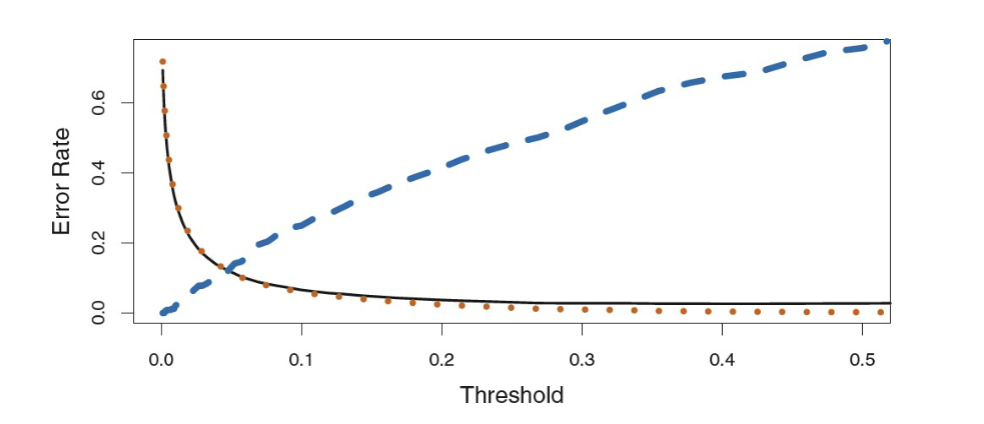
\includegraphics[width=0.6\textwidth]{Screenshot 2025-06-03 at 3.15.30 PM.png}
\end{figure}

\begin{itemize}
    \item This shows how changing the threshold changes the error rates. 0.5 means anything > 0.5 gets put as TRUE, anything below gets put as FALSE
    \item same for all values $\in (0,1)$
\end{itemize}

\subsubsection{ROC curve:}
\begin{figure}[h!]
    \centering
    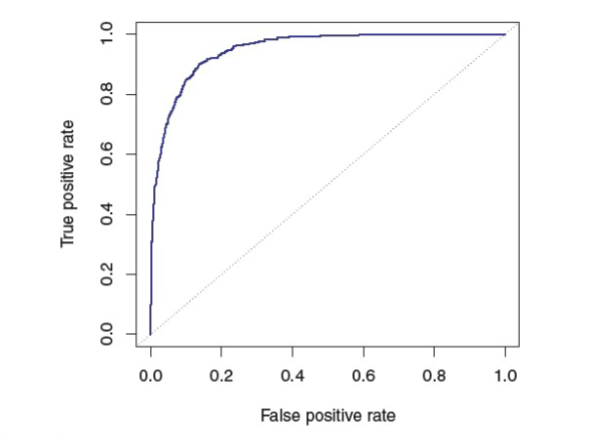
\includegraphics[width=0.6\textwidth]{ROC curve.png}
\end{figure}

\subsection{Type 1 and Type 2 error}

\begin{table}[ht]
  \centering
  \begin{tabular}{@{} l  l  l @{}}
    \toprule
    Name                & Definition      & Synonyms                                           \\
    \midrule
    False Pos.\ rate    & $\mathrm{FP}/N$ & Type I error,\; $1\!-\!\text{Specificity}$         \\
    True Pos.\ rate     & $\mathrm{TP}/P$ & $1\!-\!\text{Type II error},\;\text{power},\;\text{sensitivity},\;\text{recall}$ \\
    Pos.\ Pred.\ value  & $\mathrm{TP}/P^{*}$ & Precision,\; $1\!-\!\text{false discovery proportion}$ \\
    Neg.\ Pred.\ value  & $\mathrm{TN}/N^{*}$ &                                                    \\
    \bottomrule
  \end{tabular}
\end{table}


\subsection{Quadratic discriminant analysis}
\begin{itemize}
    \item The quadratic discriminant analysis (QDA) assumes that each class has its own covariance matrix. That is, it assumes that an observation from the $k$th class is of the form $\mathbf{X} \sim N(\mathbf{\mu}_k,\mathbf{\Sigma}_k)$ where $\mathbf{\Sigma}_k$ is a covariance matrix of the kth class.
    \item Hence applying this to Bayes theorem.
    \begin{align*}
    \delta_k(x)
    &= 
    -\tfrac{1}{2}\,\mathbf{x}\,\mathbf{\Sigma}_k^{-1}\,x^\top
    \;+\;\mathbf{x}\,\mathbf{\Sigma}_k^{-1}\,\mathbf{\mu}_k^\top
    \;-\;\tfrac{1}{2}\,\mathbf{\mu}_k\,\mathbf{\Sigma}_k^{-1}\,\mathbf{\mu}_k^\top
    \;-\;\tfrac{1}{2}\,\log\lvert \mathbf{\Sigma}_k\rvert
    \;+\;\log(\pi_k)\,. 
\end{align*}
\end{itemize}

\subsection{LDA vs QDA}
\begin{itemize}
    \item given $p$ predictors, estimating a covariance matrix requires $\frac{p (1 - p)}{2}$ parameters. QDA estimates a total of $K \frac{p(1-p)}{2}$ parameters. LDA only needs to estimate a single covariance matrix. Therefore, LDA is a much less flexible classifier than QDA, which leads to lower variance
    \item If LDA's assumption on common covariance matrix is not appropriate, then it would result in higher bias
    \item LDA tends to be a better bet than QDA if there are relatively few training observations and so reducing variance is crucial.
    \item QDA is recommended if the training set is very large, or if the assumption of a common covariance matrix for the K classes is clearly untenable
\end{itemize}


\begin{figure}[h!]
    \centering
    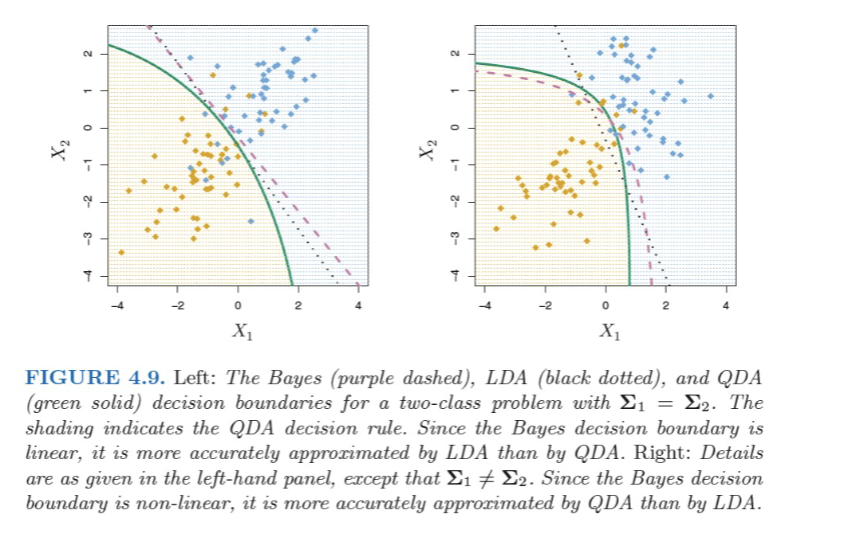
\includegraphics[width=0.6\textwidth]{LDA QDA.png}
\end{figure}

\subsection{K nearest neighbours (KNN)}

\begin{itemize}
    \item KNN works for regression and classification
    \item It uses the closest K observations in the neighbourhood of a given observation to predict the class this observation belongs to.
    \item Given a positive integer K and $\mathbf{x}_0$
    \begin{enumerate}
        \item For each observation $\mathbf{x}_i, i = 1,2,...,n$ in the training data set
        \begin{itemize}
            \item calculate the distance between $\mathbf{x}_0$ and $\mathbf{x}_i$ which is denoted by $D_i = ||\mathbf{x}_0 - \mathbf{x}_i||$
            \item Add $D_i$ and the index $i$ to an ordered collection
        \end{itemize}
        \item Sort through the ordered collection of distances and indices from smallest to largest by the distances D and the first K indices appearing in the list, denotes by $N_0$, point out the K points closest to $\mathbf{x}_0$ in the training data.
        \item Find $y_i$ for all $i \in N_0$ and identify the majority of the voting class, which is the predicted class for the test observations $\mathbf{x_0}$
    \end{enumerate}
\end{itemize}


\begin{figure}[h!]
    \centering
    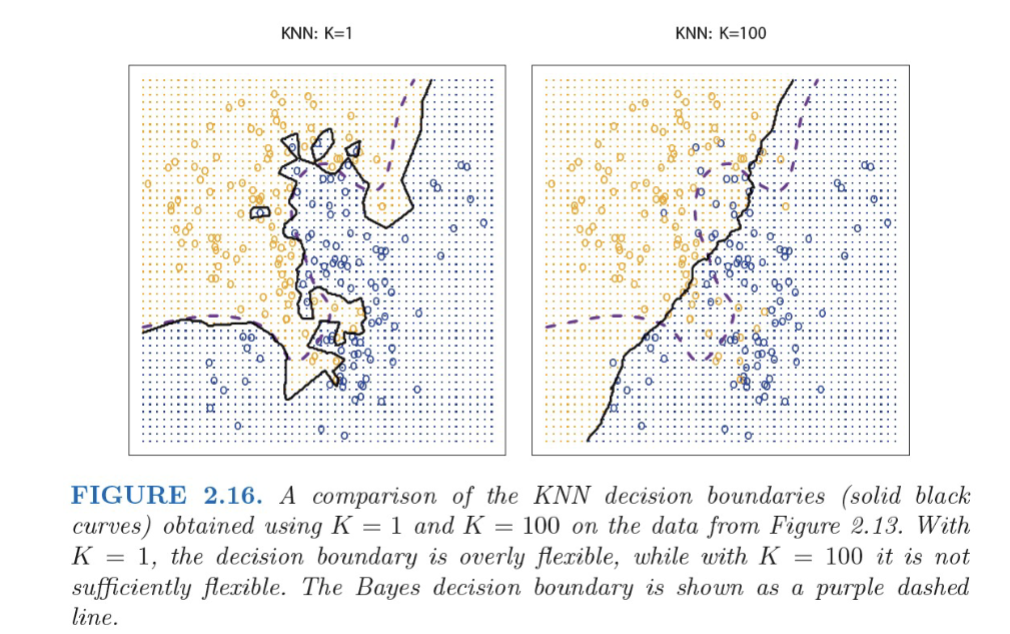
\includegraphics[width=0.6\textwidth]{KNN.png}
\end{figure}


\subsubsection{optimising K}
\begin{itemize}
    \item We must optimise K in order to get the best performance of the model.
    \item K effects the flexibility.
    \item The true decision boundary is shown by the dashed line
\end{itemize}


\subsubsection{Pros and Cons of CV}
\begin{itemize}
    \item + The algorithm is simple and easy to implement
    \item + There is no need to build a model, tune several parameters, or make additional assumptions.
    \item + The algorithm is versatile. It can be used for classification and regression.
    \item - The algorithm gets much slower as n and/or p increases
\end{itemize}

\subsection{Comparisons}
\subsubsection{Logistic regression Vs LDA}
\begin{itemize}
    \item Logistic regression and LDA methods are quite similar. 
    \item In a two-class setting with $p = 1$ and let $p_1(x)$ and $p_2(x) = 1 - p_1(x)$ be the probability that the observation X = x belongs to class 1 and class 2.
    \item In LDA
    \begin{equation*}
        \log(\frac{p_1(x)}{1 - p_1(x)}) = c_0 + c_1 x
    \end{equation*}
    \item In logistic regression
    \begin{equation*}
        \log(\frac{p_1(x)}{1 - p_1(x)}) = \beta_0 + \beta_1 x
    \end{equation*}
\end{itemize}

\subsubsection{KNN, QDA, logistic regression, LDA}
\begin{itemize}
    \item KNN is a completely non-parametric method, and no assumptions are needed about the shape of the decision boundary
    \item When the decision boundary is highly non-linear, KNN is likely to outperform LDA and logistic regression
    \item On the other hand, KNN doesn't tell us which predictors are important: no inference results for KNN
    \item QDA serves as a compromise by assuming a quadratic decision boundary. Though not as flexible as KNN, QDA can perform better in the presence of a limited number of training observations, as it does make some assumptions about the form of decision boundary.
\end{itemize}



\subsubsection{6 scenarios of comparison (let p = 2)}

\begin{itemize}
    \item S1: There were 20 training observations in each of the two classes. Observations within each class were uncorrelated normal r.v's with a different mean in each class.
    \begin{itemize}
        \item This scenario suits LDA very well. (LDA perfroms well).
        \item The performance of logistic regression is similar to LDA, and QDA is slightly worse as it is more flexible than LDA.
        \item KNN didn't perform well since it didn't have much advantage on bias reduction in this linear decision boundary case.
    \end{itemize}
    \item S2: Same as S1 except within each class the two predictors had correlation of -0.5
    \begin{itemize}
        \item Performances are similar to model 1
    \end{itemize}
    \item S3: Generated $X_1$ and $X_2$ from a t-distribution, with 50 observations per class, the decision boundary is still linear, and so fit into the logistic regression framework
    \begin{itemize}
        \item In this setting the decision boundary is still linear so logstic regression worked very well
        \item Since the normal assumption was not met, LDA worked slightly worse than logistic regression.
        \item The QDA method deteriorated considerably as a consequence of non-normality
        \item KNN in general still didn't perform well. However KNN-CV improved moderately
    \end{itemize}
    \item S4: The data were generated from a normal distribution, with a correlation of 0.5 between the predictors in the first class, and correlation of -0.5 between the predictors in the second class.
    \begin{itemize}
        \item This scenario corresponds to the QDA assumption, and results in a quadratic decision boundary. Therefore, QDA outperforms all other methods.
    \end{itemize}
    \item S5: Within each class, the observations were generated from a normal distribution with uncorrelated predictors. However, the responses were sampled from the logistic function using $X_1^2$, $X_2^2$, and $X1 \text{X} X2$ as predictors. Consequently, there is a quadratic decision boundary.
    \begin{itemize}
        \item Again, QDA outperforms the linear methods, and the KNN-CV had an improved performance as the data became more complex.
    \end{itemize}
    \item S6: Details are as in S5, but the responses were sampled from a more complicated non-linear function.
    \begin{itemize}
        \item As a result, even the QDA couldn't adequately model the data. In this case, KNN-CV method performed better than the others. KNN-1 performed poorly, indicating that even when the data exhibits a complex non-linear relationship, a non-parametric method like KNN can still give poor results if the level of smoothness is not chosen correctly.
    \end{itemize}
\end{itemize}

\subsection{Classification in R}

\begin{itemize}
    \item First use \texttt{pairs} to see the relationship between variables
    \item By making a binary response a colour, R will colour all values that adhere to the indicator 
\end{itemize}

\begin{lstlisting}
library(glmnet)
glm.fits=glm(Direction~Lag1+Lag2+Lag3+Lag4+Lag5+Volume,data=Smarket,family=binomial)
#family = binomial  performs logistic regression
summary(glm.fits)
coef(glm.fits)
summary(glm.fits)$coef
summary(glm.fits)$coef[,4] #Showing the associated p-values only
glm.probs=predict(glm.fits,type="response") #type="response" returns P(Y=1|X)
glm.probs[1:10] #All responses around 0.5 since >0.5 = up, <0.5 = down
glm.pred=rep("Down",1250) #creating 1250 Down elements
glm.probs>.5 #see what we have in this 
glm.pred[glm.probs>.5]="Up" #transforming those elements whose prob.>0.5 to Up
table(glm.pred,Direction) #The confusion matrix
mean(glm.pred==Direction) #rate of correct predictions, i.e. 1-training error rate
mean(glm.pred!=Direction)#training error rate
\end{lstlisting}

\begin{lstlisting}
train=(Year<2005)
Smarket.2005=Smarket[!train,] #selecting observations in 2005 (! = not in, flips TRUE to FALSE)
dim(Smarket.2005)
Direction.2005=Direction[!train]

# Fit the logistic regression using training set
glm.fits=glm(Direction~Lag1+Lag2+Lag3+Lag4+Lag5+Volume,
             data=Smarket,family=binomial,subset=train)
# Predict using test set
glm.probs=predict(glm.fits,Smarket.2005,type="response")
glm.pred=rep("Down",252) # 252 since Dim(Smarket.2005) = 252
glm.pred[glm.probs>.5]="Up" #if glm.probs is >0.5 replace the corresponding value in glm.pred
table(glm.pred,Direction.2005) #True pos, True neg, False pos, False neg
#True pos and False neg are good!
mean(glm.pred==Direction.2005) #rate of correct predictions
mean(glm.pred!=Direction.2005) #test error rate

#Predicted down and went down
sum(glm.pred==Direction.2005 & glm.pred=="Down") 

#True positive / true positive + false negative aka Correct up predictions / Actual up days
sum(glm.pred==Direction.2005 & glm.pred=="Up")/sum(Direction.2005=="Up")

\end{lstlisting}

\begin{lstlisting}
#REMOVED WEAKEST PREDICTORS
glm.fits=glm(Direction~Lag1+Lag2,data=Smarket,family=binomial,subset=train)
glm.probs=predict(glm.fits,Smarket.2005,type="response")
glm.pred=rep("Down",252)
glm.pred[glm.probs>.5]="Up"
table(glm.pred,Direction.2005)

#mean computes the overall accuracy of the model Up/Down matched what actually happened
mean(glm.pred==Direction.2005)

#Sensitivity
sum(glm.pred==Direction.2005 & glm.pred=="Up")/sum(Direction.2005=="Up")
\end{lstlisting}

\begin{lstlisting}
    # Logistic on Y with multiple classes
    # Suppose df has Y1, Y2, Y3 all 0/1, plus predictors X1, X2
yrs <- c("Y1","Y2","Y3")
fits <- lapply(yrs, function(y) {
  glm(
    formula = reformulate(c("X1","X2"), response = y),
    data     = df,
    family   = binomial()
  )
})
names(fits) <- yrs

# Summaries:
lapply(fits, summary)

\end{lstlisting}



\pagebreak

\begin{center}
    \Large{Chapter 5: Cross-Validation and the Bootstrap}
\end{center}

\section{Chapter 5}

\subsection{Cross-Validation}

\subsubsection{Resampling Methods}
\begin{itemize}
    \item Cross-validation and the Bootstrap are resampling methods used to assess model performance and estimate uncertainty.
\end{itemize}

\subsubsection{Training Error}
\begin{itemize}
    \item \textbf{Training error:} computed by applying the learning method to the same observations used for training.
    \item Typically lower than test error, since the model has seen this data.
\end{itemize}

\subsubsection{Test Error}
\begin{itemize}
    \item \textbf{Test error:} average error from using the method to predict new observations not used in training.
    \item Reflects performance on unseen data and helps detect overfitting.
    \item Test error = Bias$^2$ + Variance + Irreducible error; aim to minimize overall test error.
    \item Overfitting increases the test error.
\end{itemize}

\begin{figure}[h!]
    \centering
    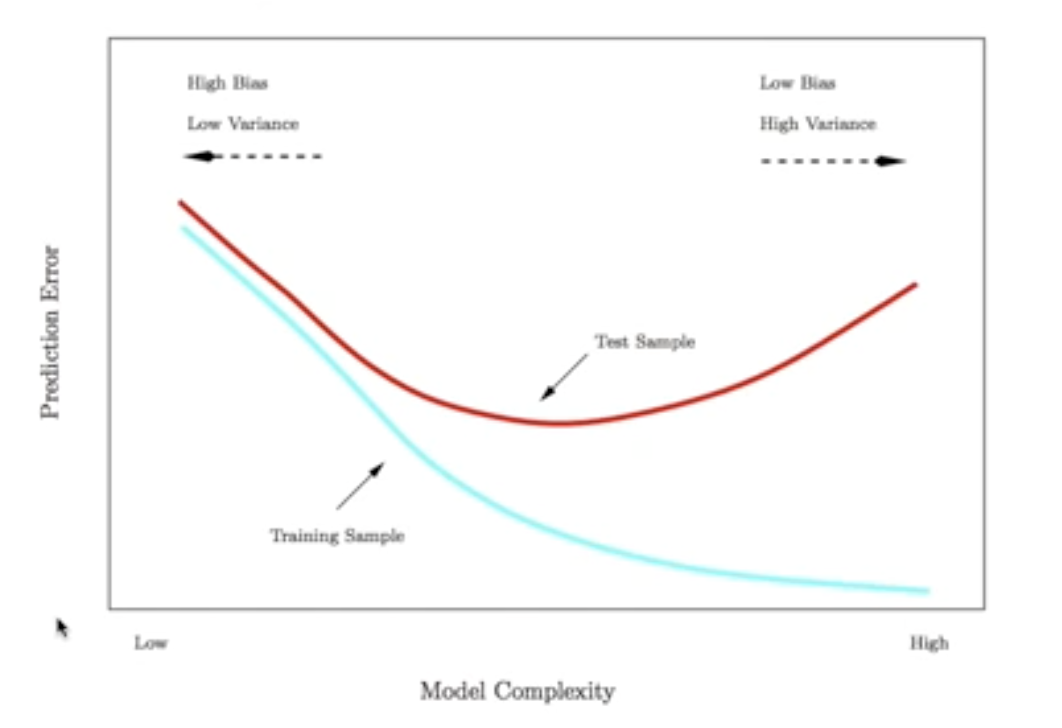
\includegraphics[width=0.6\textwidth]{training vs test error.png}
\end{figure}

\subsubsection{Prediction-error estimates}
\begin{itemize}
    \item The best solution is to designate a very large test set - however this is not always available.
    \item Some methods like mathematical adjustment to the training error rate in order to estimate the test error rate. These include the Cp statistic, AIC and BIC.
\end{itemize}

\subsubsection{Validation-Set Approach}
\begin{itemize}
    \item Randomly split data into a training set and a validation set.
    \item Fit the model on the training set.
    \item Evaluate the fitted model on the validation set by computing MSE.
    \item Provides an estimate of test error.
\end{itemize}

\begin{figure}[h!]
    \centering
    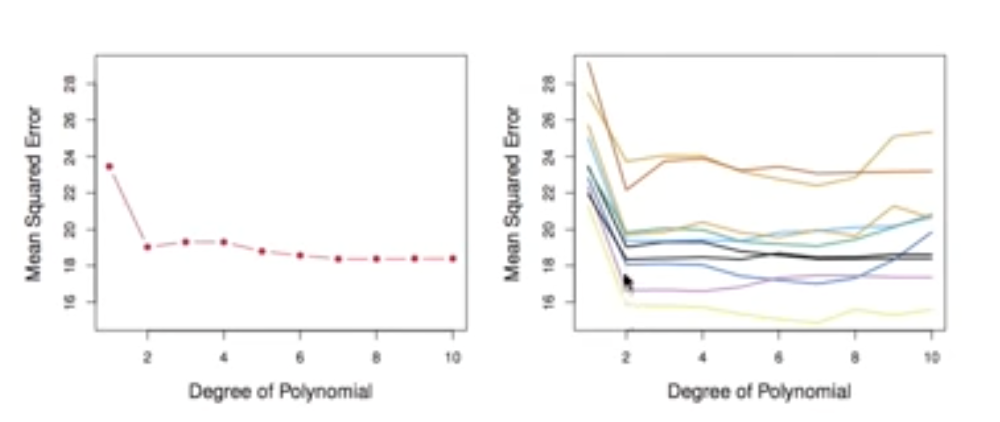
\includegraphics[width=0.6\textwidth]{splitting data for validation.png}
\end{figure}
\begin{itemize}
    \item The difference in MSE occurs due to splitting the data, here we can see that fitting a polynomial with degree 2 is the best.
\end{itemize}

\subsubsection{Drawbacks of validation}
\begin{itemize}
    \item The validation estimate of the test error can be highly variable, depending on precisely which observations are included in the training set and which observations are included in the validation set.
    \item In the validation approach, only a subset of the observations - those that are included in the training set rather than in the validation set - are used to fit the model.
\end{itemize}

\subsubsection{Leave-One-Out and k-Fold Cross-Validation}
\begin{itemize}
    \item \textbf{LOOCV:} each training set uses $n-1$ observations; average validation error across all splits.
    \item \textbf{k-Fold CV:} partition data into $k$ subsets; use $k-1$ for training and 1 for validation, rotate through all folds.
    \item Since each training fold is only $(k-1)/k$ the size of the full data, CV error estimates can be biased upward.
    \item Bias is minimised when $k=n$ (LOOCV), but variance is high.
    \item Common practice: $k=5$ or $10$ to balance bias and variance.
    \item High k means lots of training data hence high variance low bias, low k means not as much training data hence high bias low variance.
    \item LOOCV has high variance since you are only testing on one point which makes the variance of the average of the $n$ is high.
    \item Let the K parts be $C_1, C_2, ..., C_k$ CV error rate:
    \begin{equation*}
        \mathrm{CV}_{(K)} = \sum_{k=1}^K \frac{n_k}{n} \mathrm{MSE}_k
    \end{equation*}
    where the $\frac{n_k}{n}$ is averaging the different CV lines that have been produced by different partitions in the data.
    \item MSE$_k = \sum_{i\in C_k} (y_i - \hat{y}_i)^2 /n_k$, and $\hat{y}_y$ is the fit for observation $i$, obtained from the data with part $k$ removed.
    \item For LOOCV
    \begin{equation*}
        \mathrm{CV}_{(n)} = \frac{1}{n}\sum_{i=1}^n (\frac{y_i - \hat{y}_i}{1 - h_i})^2
    \end{equation*}
    \item Where $\hat{y}_i$ is the ith fitted value from the original least squares fit. and $h_i$ is the leverage.
    \item 10-fold CV reduces variability.
    \item Since each training set is only (K-1)/K as big as the original training set, the estimates of prediction error will be biased upward.
    \begin{itemize}
        \item This bias minimised when K = n (LOOCV), but this estimate has high variance
    \end{itemize}
\end{itemize}

\pagebreak

\begin{table}[ht]
  \centering
  \begin{tabular}{@{}p{3cm}p{5.5cm}p{5.5cm}@{}}
    \toprule
    \textbf{Aspect} & \textbf{K-fold (e.g.\ \(K=5\) or \(10\))} & \textbf{LOOCV (\(K=N\))} \\
    \midrule
    \textbf{Estimate bias} &
      Tends to have slightly higher bias (since training sets are smaller) &
      Lower bias (almost uses full data each time) \\
    \addlinespace
    \textbf{Estimate variance} &
      Lower variance of the error estimate (fold averages smooth out fluctuations) &
      Higher variance (each held-out point can exert large influence) \\
    \addlinespace
    \textbf{Computation} &
      \(K\) model fits &
      \(N\) model fits (often much larger) \\
    \addlinespace
    \textbf{Use case} &
      Default choice for most practical problems &
      Useful for very small datasets or when maximal data utilization is critical \\
    \bottomrule
  \end{tabular}
\end{table}
\paragraph{When to choose which?}
Use \emph{5- or 10-fold CV} by default, as it balances reliable error estimation with reasonable computational cost. Turn to \emph{LOOCV} only when your dataset is very small and you need to train on as much data as possible for each fit—keeping in mind the substantially higher computation and potentially noisier (high-variance) error estimates.

\subsection{Bias–Variance Trade‐off for \(k\)-fold CV}

We shall compare the performance of the CV methods introduced so far on:
\begin{itemize}
  \item \textbf{Bias}:  
    According to the amount of data used in fitting, clearly the validation set approach has the highest bias, and LOOCV has the lowest.
  \item \textbf{Variance}:  
    \(k\)-fold CV tends to have lower variance than LOOCV if \(k<n\). This is because LOOCV is averaging outputs of \(n\) highly correlated (i.e.\ more overlap) fitted models, while \(k\)-fold CV is averaging \(k\) less correlated (i.e.\ less overlap) outputs.
  \item \textbf{Overall}:  
    \(k\)-fold CV tends to give a more accurate estimate of the test error rate than does LOOCV.
\end{itemize}

Bias–variance trade‐off: there is a bias–variance trade‐off associated with the choice of \(k\) in \(k\)-fold CV. Typically we use \(k=5\) or \(k=10\) as they have been empirically shown to have less high‐bias and high‐variance issues. It can be easily applied to a wide range of statistical learning methods, including some for which a measure of variability is otherwise difficult to obtain and is not automatically output by statistical software.









\subsection{The Bootstrap}
\begin{itemize}
    \item The bootstrap quantifies uncertainty by resampling with replacement from the original dataset.
    \item \textbf{Example:} Investing a sum in assets $X$ and $Y$.
    \begin{itemize}
        \item Allocate fraction $\alpha$ to $X$ and $1-\alpha$ to $Y$.
        \item Portfolio variance: $\mathrm{Var}(\alpha X + (1-\alpha)Y)$.
        \item Optimal $\alpha^*$ that minimizes variance:
        \[
            \alpha^* = \frac{\mathrm{Var}(Y) - \mathrm{Cov}(X,Y)}{\mathrm{Var}(X) + \mathrm{Var}(Y) - 2\,\mathrm{Cov}(X,Y)}
        \]
        \item True variances and covariance unknown; estimate via bootstrap.
    \end{itemize}
    \item Generate many bootstrap samples (same size as original), compute estimator for each, and assess variability.
    Estimated standard deviation of CV$_K$ is 
    \begin{equation*}
        \hat{\mathrm{CV}}_K = \sqrt{\sum_{k=1}^K (\mathrm{Err}_k - \bar{\mathrm{Err}_k})^2 / (K-1)}
    \end{equation*}
    \item THE BOOTSTRAP CAN HAVE REPLACEMENTS
\end{itemize}

\subsubsection{Bootstrap Extended}
\begin{itemize}
    \item Replace population distribution with empirical distribution $\hat{p}$.
    \item Use bootstrap samples to construct confidence intervals and other measures of estimator accuracy.
\end{itemize}


\begin{lstlisting}
# The Validation Set Approach

library(ISLR)

# First way of dividing data
set.seed(1)
train=sample(392,196) #generate training index subset
attach(Auto)
lm.fit=lm(mpg~horsepower,data=Auto,subset=train)
mean((mpg-predict(lm.fit,Auto))[-train]^2) # test MSE 
mean((mpg[-train]-predict(lm.fit,Auto[-train,]))^2) # alternative
# quadratic regression
lm.fit2=lm(mpg~poly(horsepower,2),data=Auto,subset=train)
mean((mpg-predict(lm.fit2,Auto))[-train]^2)
# polynomial regression
lm.fit3=lm(mpg~poly(horsepower,3),data=Auto,subset=train)
mean((mpg-predict(lm.fit3,Auto))[-train]^2)

\end{lstlisting}

\pagebreak

\begin{center}
    \Large{Chapter 6: Linear Model Selection and Regularization}
\end{center}

\section{Chapter 6: Linear Model Selection and Regularization}

\subsection{Subset selection}

\begin{itemize}
    \item Why consider alternatives to least squares
    \begin{itemize}
        \item Prediction accuracy: especially when $p > n$ to control variance
        \item Model interpret ability: By removing irrelevant features that is by setting the corresponding coefficient estimates to zero we can obtain a model that is more easily interpreted.
    \end{itemize}
\end{itemize}
\subsubsection{Three classes of methods}

\begin{itemize}
  \item \textbf{Subset Selection.}
    We identify a subset of the $p$ predictors that we believe to be related to the response.
    We then fit a model using least squares on the reduced set of variables.
  \item \textbf{Shrinkage.}
    We fit a model involving all $p$ predictors, but the estimated coefficients are shrunken
    towards zero relative to the least squares estimates.
    This shrinkage (also known as regularization) has the effect of reducing variance
    and can also perform variable selection.
  \item \textbf{Dimension Reduction.}
    We project the $p$ predictors into an $M$–dimensional subspace, where $M < p$.
    This is achieved by computing $M$ different linear combinations, or projections,
    of the variables. Then these $M$ projections are used as predictors to fit
    a linear regression model by least squares.
\end{itemize}


\subsubsection{Best subset selection}

\begin{itemize}
    \item Let $M_0$ denote the null model, which contains no predictors. This model smply predicts the sample mean for each observation.
    \item For $k = 1,2,...p$
    \begin{itemize}
        \item Fit all $\binom{p}{k}$ models that contains exactly $k$ predictors.
        \item Pock the best among these $\binom{p}{k}$ models and call it $M_k$. Best is defined as having the smallest RSS, or equivalently largest $R^2$
    \end{itemize}
    \item Select a single best model from among $M_0,...,M_p$ using cross-validation prediction error, $C_p, (AIC) , (BIC)$ or adjusted $R^2$ 
\end{itemize}

\subsubsection{Best Subset selection in R}
\begin{lstlisting}
#Clean the data
sum(is.na(Hitters$Salary))
Hitters=na.omit(Hitters)
dim(Hitters)
sum(is.na(Hitters))

# Best Subset Selection
library(leaps)
# Build best subsets with up to 8 predictors (default option)
regfit.full=regsubsets(Salary~.,Hitters)
summary(regfit.full)
# Build best subsets with up to 19 predictors
regfit.full=regsubsets(Salary~.,data=Hitters,nvmax=19)
summary(regfit.full)
reg.summary=summary(regfit.full)
names(reg.summary)
reg.summary$rsq
\end{lstlisting}

\subsection{Stepwise Selection}

\begin{itemize}
    \item When p is large best subset selection does not work very well since there is usually $\approx 40$ predictors per dataset. Hence we cant really use it unless p is quite small
    \item To avoid fitting too hard it can be better to not use best subset selection. Hence forward selection is good.
    \item Best subset selection is good for $p \leq 10$
\end{itemize}

\subsubsection{Forward Stepwise Selection}
\begin{itemize}
    \item Forward stepwise selection begins with a model containing no predictors, and then adds predictors to the model one at a time, until all predictors are in the model.
    \item At each step the variable that gives the greatest additional improvement to the fit is added to the model.
    \begin{enumerate}[label=\arabic*.]
  \item Let $\mathcal M_0$ denote the \emph{null} model, which contains no predictors.
  
  \item For $k = 0,\dots,p-1$:
    \begin{itemize}
      \item Consider all $p - k$ models that augment the predictors in $\mathcal M_k$ with one additional predictor.
      \item Choose the \emph{best} among these $p - k$ models, and call it $\mathcal M_{k+1}$. Here “best” is defined as having smallest RSS or highest $R^2$.
    \end{itemize}
  \item Select a single best model from among $\mathcal M_0,\dots,\mathcal M_p$ using cross-validated prediction error, $C_p$ (AIC), BIC, or adjusted $R^2$.
    \end{enumerate}
    \item We cant use RSS or $R^2$ since they all have different sizes.
    \item Forward selection has a computational advantage over best subset selection since best subset selection is computing $2^p$ models whereas forward stepwise is considering $\approx p^2$models
    \begin{equation*}
        RSS_{\mathrm{best subset selection}} \geq RSS_{\mathrm{forward stepwise slection}}
    \end{equation*}
\end{itemize}

\subsubsection{Forward Stepwise Selection in R}
\begin{lstlisting}
regfit.fwd=regsubsets(Salary~.,data=Hitters,nvmax=19,method="forward")
summary(regfit.fwd)
\end{lstlisting}

\subsubsection{Backward Stepwise Selection}
\begin{itemize}
    \item For backward stepwise selection we begin with the full least squares model containing all $p$ predictors, and then iteratively removes least useful predictor one at a time.
\end{itemize}

\begin{itemize}
  \item Let $\mathcal M_p$ denote the \emph{full} model, which contains all $p$ predictors.

  \item For $k = p, p-1, \dots, 1$:
    \begin{itemize}
      \item Consider all $k$ models that contain all but one of the predictors in $\mathcal M_k$, for a total of $k-1$ predictors.
      \item Choose the \emph{best} among these $k$ models, and call it $\mathcal M_{k-1}$. Here “best” is defined as having smallest RSS or highest~$R^2$.
    \end{itemize}

  \item \textbf{Select a single best model} from among $\mathcal M_0, \dots, \mathcal M_p$ using cross-validated prediction error, $C_p$ (AIC), BIC, or adjusted~$R^2$.
  \item One again considers $p^2$ models
  \item Searches exactly $1 + p(p+1)/2$ models
\end{itemize}

\subsubsection{Backward Stepwise Selection in R}
\begin{lstlisting}
regfit.bwd=regsubsets(Salary~.,data=Hitters,nvmax=19,method="backward")
summary(regfit.bwd)
\end{lstlisting}

\subsubsection{Choosing the Optimal Model}
\begin{itemize}
    \item The model containing all of the predictors will always have the smallest RSS and the largest R$^2$ since these quantities are related to the training error.
    \item We wish to choose a model with a low test error, not training error!
    \item Therefore RSS and R$^2$ are not suitable for selecting the best model along with different numbers of parameters
\end{itemize}

\subsection{Estimating Test error}
\begin{itemize}
  \item We can \emph{indirectly} estimate test error by making an \emph{adjustment} to the training error to account for the bias due to overfitting.
  \item We can \emph{directly} estimate the test error, using either a validation‐set approach or a cross‐validation approach.
\end{itemize}

\subsubsection{Mallow's C$_p$}
\begin{itemize}
    \item Mallow's C$_p$
    \begin{equation*}
        C_p = \frac{1}{n}(\mathrm{RSS} + 2 d \hat{\sigma}^2)
    \end{equation*}
    where $d$ is the total no. of parameters used and $\hat{\sigma}^2$ is an estimate of the variance of the error $\epsilon$ associated with each response measurement.
    \item We want the smallest C$_p$
\end{itemize}

\subsubsection{C$_p$ in R}

\begin{lstlisting}
which.min(reg.summary$cp)
points(10,reg.summary$cp[10],col="red",cex=2,pch=20)
\end{lstlisting}

\subsubsection{AIC}
\begin{itemize}
    \item Aikike Information Criterion (AIC) is defined for a large class of models fit by maximum likelihood:
    \begin{equation*}
        \mathrm{AIC} = -2\log(L) + 2\cdot d
    \end{equation*}
    where $L$ is the maximised value of the likelihood function for the estimated model. ($-2\log(L) = \frac{\mathrm{RSS}}{\hat{\sigma}^2}$)
\end{itemize}

AIC and C$_p$ are proportional to eachother. (THe same thing for linear models) 


\subsubsection{BIC}
\begin{itemize}
    \item Bayesian Information Criterion (BIC) 
    \begin{equation*}
        \mathrm{BIC} = \frac{1}{n} (\mathrm{RSS} + \log(n) d \hat{\sigma}^2)
    \end{equation*}
    \item Like C$_p$ BIc will tend to take smaller values for a model with low test error. Hence we select the model with smallest BIC
    \item BIC replaces the $2d \hat{\sigma}^2$ used in C$_p$ with a $\log(n) d \hat{\sigma}^2$ where $n$ is the number of observations.
    \item Since $\log(n) > 2$ for any $n > 7$, teh BIC statistic generally places a heavier pentalty on models with many variables, and hence results in the selection of smaller models than C$_p$.
\end{itemize}
\subsubsection{BIC in R}

\begin{lstlisting}
plot(reg.summary$bic,xlab="Number of Variables",ylab="BIC",type="l")
which.min(reg.summary$bic)
points(which.min(reg.summary$bic),reg.summary$bic[which.min(reg.summary$bic)],
        col="red",cex=2,pch=20)
\end{lstlisting}



\subsubsection{Adjusted R$^2$}

\begin{itemize}
    \item Adjusted R$^2$
    \begin{equation*}
        \mathrm{Adusted } \; R^2 = 1 - \frac{RSS/(n-d-1)}{TSS/(n-1)}
    \end{equation*}
    Where $TSS = \sum_{i} (y_i - \bar{y})^2$ (Total sum of squares)
    \item A large value of Adjusted R$^2$ indicated a model with small test error.
    \item Maximising the adjusted R$^2$ is equivalent to minimizing $\frac{\mathrm{RSS}}{n-d-1}$. While RSS always decreases as the number of variables in the model increases, $\frac{\mathrm{RSS}}{n-d-1}$ may increase or decrease due too the presence of $d$ in the denominator.
    \item Unlike R$^2$ statistic, the adjusted R$^2$ statistic pays a price for the inclusion of unnecessary variables in the model.
\end{itemize}

\subsubsection{Adjusted R$^2$ in R}
\begin{lstlisting}
plot(reg.summary$adjr2,xlab="Number of Variables",ylab="Adjusted Rsq",type="l")
# Find out the case with maximal adjusted R^2
which.max(reg.summary$adjr2)
# [1] 11
# Draw points in the latest plot
points(11,reg.summary$adjr2[11], col="red",cex=2,pch=20)
\end{lstlisting}


\subsection{Validation and Cross-Validation}

\begin{itemize}
  \item Each of the procedures returns a sequence of models $M_k$ indexed by model size $k = 0, 1, 2, \dots$.  Our job here is to select $\hat{k}$.  Once selected, we will return model $M_{\hat{k}}$.
  \item We compute the validation‐set error or the cross‐validation error for each model $M_k$ under consideration, and then select the $k$ for which the resulting estimated test error is smallest.
  \item This procedure has an advantage relative to AIC, BIC, $C_p$, and adjusted $R^2$, in that it provides a direct estimate of the test error, and \emph{doesn't} require an estimate of the error variance $\sigma^2$.
  \item It can also be used in a wider range of model‐selection tasks, even in cases where it is hard to pinpoint the model degrees of freedom (e.g.\ the number of predictors in the model) or hard to estimate the error variance $\sigma^2$.
\end{itemize}

\subsubsection{Validation method in R}

\begin{lstlisting}
# Create training set and test test
set.seed(1)
train=sample(c(TRUE,FALSE), nrow(Hitters),rep=TRUE)
test=(!train)
regfit.best=regsubsets(Salary~.,data=Hitters[train,],nvmax=19)

# direct method of finding the best model

test.mat=model.matrix(Salary~.,data=Hitters[test,])
val.errors=rep(NA,19)

coef3=coef(regfit.best,id=3)
coef3
View(test.mat[,names(coef3)])

#This function compares the test MSE for each number of predictors 1:19 and stores
#it as val.errors. we want the minimum.
for(i in 1:19){
  coefi=coef(regfit.best,id=i)
  pred=test.mat[,names(coefi)]%*%coefi
  val.errors[i]=mean((Hitters$Salary[test]-pred)^2)
}
val.errors
which.min(val.errors)
coef(regfit.best,which.min(val.errors))

# best is 7 for seed 1 and 9 for seed 10.


# Create the function of prediction and find the best model

predict.regsubsets=function(object,newdata,id,...){ #... allows for other arguments to be passed into the function
  form=as.formula(object$call[[2]])
  mat=model.matrix(form,newdata)
  coefi=coef(object,id=id)
  xvars=names(coefi)
  mat[,xvars]%*%coefi
}

val.errors=rep(NA,19)
for(i in 1:19){
  pred=predict.regsubsets(regfit.best,Hitters[test,],id=i) #can also use predict()
  val.errors[i]=mean((Hitters$Salary[test]-pred)^2)
}
val.errors
which.min(val.errors)
coef(regfit.best,which.min(val.errors))

# Obtain the best subset model using the full data and CV selected id

regfit.best=regsubsets(Salary~.,data=Hitters,nvmax=19)
coef(regfit.best,which.min(val.errors))
\end{lstlisting}

\subsubsection{K-fold Cross-Validation method in R}
\begin{lstlisting}
k=10
set.seed(1)
folds=sample(1:k,nrow(Hitters),replace=TRUE)
cv.errors=matrix(NA,k,19, dimnames=list(NULL, paste(1:19)))

for(j in 1:k){
  best.fit=regsubsets(Salary~.,data=Hitters[folds!=j,],nvmax=19)
  for(i in 1:19){
    pred=predict(best.fit,Hitters[folds==j,],id=i)
    cv.errors[j,i]=mean( (Hitters$Salary[folds==j]-pred)^2)
  }
}
mean.cv.errors=apply(cv.errors,2,mean)
mean.cv.errors
plot(mean.cv.errors,type='b')

# Obtain the best subset model using the full data and CV selected id
reg.best=regsubsets(Salary~.,data=Hitters, nvmax=19)
coef(reg.best,10)

\end{lstlisting}


\subsection{Shrinkage Methods}

\subsubsection{Ridge regression}
\begin{itemize}
    \item Recall that the least squares fitting procedure estiamtes $\beta_0, \beta_1, ..., \beta_p$ using the values to minimize
    \begin{equation*}
        \mathrm{RSS} = \sum_{i=1}^n (y_i - \beta_0 - \sum_{j=1}^p \beta_j x_{ij})^2
    \end{equation*}
    \item In contrast, te ridge regression coefficents estimates $\hat{\beta}^R$, the values that minimize
    \begin{equation*}
        \sum_{i=1}^n (y_i - \beta_0 - \sum_{j=1}^p \beta_j x_{ij})^2 + \lambda \sum_{j=1}^p \beta_j^2 = \mathrm{RSS} + \lambda \sum_{j=1}^p \beta_j^2
    \end{equation*}
    where $\lambda>0$ is a tuning parameter to be determined separately.
    \item As with least squares, ridge regression seeks coefficient estimates that fit the data well, by making the residual sum of squares (RSS) small.
    \item However, the second term, 
    \[
      \lambda \sum_{j=1}^p \beta_j^2,
    \]
    called a \emph{shrinkage penalty}, is small when \(\beta_1,\dots,\beta_p\) are close to zero, and so it has the effect of \emph{shrinking} the estimates of \(\beta_j\) towards zero.
    \item When $\lambda = 0$ we are just fitting \texttt{lm} since there is no weight to the penalty term.
    \item The tuning parameter \(\lambda\) serves to control the relative impact of these two terms on the regression coefficient estimates.
    \item Selecting a good value for \(\lambda\) is critical; cross‐validation is used for this.
    \item The standard least squares coefficient estimates are \emph{scale equivariant}: multiplying \(X_j\) by a constant \(c\) simply leads to a scaling of the least squares coefficient estimates by a factor of \(1/c\).  In other words, regardless of how the \(j\)th predictor is scaled, \(X_j \beta_j\) will remain the same. 
    \item In contrast, the ridge regression coefficient estimates can change \emph{substantially} when multiplying a given predictor by a constant, due to the sum of squared coefficients term in the penalty part of the ridge regression objective function.
    \item Therefore, it is best to apply ridge regression after \emph{standardising the predictors}, using the formula
    \[
      \tilde{x}_{ij}
      = \frac{x_{ij}}
             {\sqrt{\displaystyle\frac{1}{n}\sum_{i=1}^n (x_{ij}-\bar{x}_j)^2}}.
    \]
\end{itemize}

\subsubsection{Ridge regression in R}
\begin{lstlisting}
# 1. Prepare the predictor matrix and response
library(glmnet)
x <- model.matrix(Salary ~ ., Hitters)[, -1]  # drop the intercept column
y <- Hitters$Salary

# 2. Define a grid of $\lambda$ values
grid <- 10^seq(10, -2, length = 100)

# 3 Fit the ridge regression ($\alpha$ = 0)
ridge.mod <- glmnet(x, y, alpha = 0, lambda = grid)

# 4. (Optional) Split into training and test sets
set.seed(1)
train <- sample(seq_len(nrow(x)), nrow(x) / 2)
test  <- -train
y.test <- y[test]

# 5. Predict on the test set at a chosen $\lambda$ (e.g. \lambda = 4)
pred <- predict(ridge.mod, s = 4, newx = x[test,])
mean((pred - y.test)^2) #MSE

# replace step 5 with cross-validation to choose $\lambda$ automatically
#CV is to find the best lambda, the set lambda tests a vale for lambda.

cv.out  <- cv.glmnet(x[train, ], y[train], alpha = 0)
bestlam <- cv.out$lambda.min
pred_cv <- predict(ridge.mod, s = bestlam, newx = x[test, ])
mean((pred_cv - y.test)^2) #MSE
\end{lstlisting}


\subsubsection{The Lasso}
\begin{itemize}
    \item The disadvantage of ridge regression is that it includes all p predictors in the final model
    \item The \emph{Lasso} is a relatively recent alternative to ridge regression that overcomes this disadvantage. The lasso coefficients, $\hat{\beta}^L_\lambda$ minimize the quantity
    \begin{equation*}
        \sum_{i=1}^n \biggl(y_i - \beta_0 - \sum_{j=1}^p \beta_j x_{ij}\biggr)^2
    \;+\;\lambda \sum_{j=1}^p \lvert \beta_j \rvert
    \;=\;\mathrm{RSS} \;+\;\lambda \sum_{j=1}^p \lvert \beta_j \rvert
    \end{equation*}
    \item The lasso also shrinks coefficient estimates towards zero, however in this case the $\ell_1$ penalty has the effect of forcing some coefficient estimates to be exactly zero when the tuning parameter $\lambda$ is sufficiently large.
    \item Hence like best subset selection, the lasso also performs variable selection.
    \item Same in ridge regression, selecting a good value of $\lambda$ is crucial. CV is a good choice.
\end{itemize}


\subsubsection{The lasso in R}
\begin{lstlisting}
x=model.matrix(Salary~.,Hitters)[,-1]
y=Hitters$Salary

lasso.mod=glmnet(x[train,],y[train],alpha=1,lambda=grid)
plot(lasso.mod)

# choosing lambda by cross-validation

set.seed(1)
cv.out=cv.glmnet(x[train,],y[train],alpha=1)
plot(cv.out)
bestlam=cv.out$lambda.min
lasso.pred=predict(lasso.mod,s=bestlam,newx=x[test,])
mean((lasso.pred-y.test)^2) #MSE

# fit the best case using the full data
out=glmnet(x,y,alpha=1,lambda=grid)
lasso.coef=predict(out,type="coefficients",s=bestlam)[1:20,]
lasso.coef

# showing the non-zero coefficients

lasso.coef[lasso.coef!=0]

#As expected the lasso takes predictors of 'less importance' to equal zero.
\end{lstlisting}


\subsection{Dimension Reduction Methods}
\begin{itemize}
    \item This transforms the predictors and firs a least squares model using the transformed variables. Referred to as dimension reduction methods
    \begin{itemize}
        \item Let \(Z_1, Z_2, \dots, Z_M\) represent \(M < p\) linear combinations of our original \(p\) predictors.  That is,
        \begin{equation*}
        Z_m = \sum_{j=1}^p \phi_{mj}\,X_j
        \quad\text{for}\quad m=1,\dots,M,
        \end{equation*}
    for some constants \(\phi_{m1},\dots,\phi_{mp}\).
    \item We can then fit the linear regression model
    \begin{equation*}
      y_i = \theta_0 + \sum_{m=1}^M \theta_m\,Z_{im} + \epsilon_i,
      \quad i = 1,\dots,n,
    \end{equation*}
    using ordinary least squares.
    \item Note that in model(2), the regression coefficients are given by \(\theta_0,\theta_1,\dots,\theta_M\).  If the constants \(\phi_{m1},\dots,\phi_{mp}\) are chosen wisely, then such dimension‐reduction approaches can often outperform OLS regression.
    \end{itemize}
\end{itemize}


\subsection{Principal Components Regression and Partial Least Squares}

\subsubsection{Principal Components Regression}
\begin{itemize}
    \item The first principal component is that (normalized) linear combination of the variables with the largest variance.
    \item The second principal component has largest variance, subject to being uncorrelated with the first.
    \item Hence, with many correlated original variables, we replace them with a small set of principal components that capture their joint variation.
\end{itemize}

\subsubsection{Principal Components Regression in R}
\begin{lstlisting}
library(pls)

# Split into training and test sets
set.seed(1)
train <- sample(seq_len(nrow(Hitters)), nrow(Hitters) / 2)
test  <- setdiff(seq_len(nrow(Hitters)), train)
y.test <- Hitters$Salary[test]

# Fit PCR with 10-fold CV on the training data
pcr.fit <- pcr(
  Salary ~ .,
  data       = Hitters,
  subset     = train,
  scale      = TRUE,
  validation = "CV"
)

# Plot CV MSEP to choose number of components
validationplot(pcr.fit, val.type = "MSEP")

# Replace 5 with the chosen number of components from the plot
ncomp    <- 5
pcr.pred <- predict(pcr.fit, Hitters[test, ], ncomp = ncomp)

# Test-set MSE
mean((pcr.pred - y.test)^2)
\end{lstlisting}

\subsubsection{Partial Least Squares}
\begin{itemize}
  \item PCR identifies linear combinations, or \emph{directions}, that best represent the predictors \(X_1,\dots,X_p\).
  \item These directions are identified in an \emph{unsupervised} way, since the response \(Y\) is not used to help determine the principal component directions.
  \item That is, the response does not \emph{supervise} the identification of the principal components.
  \item Consequently, PCR suffers from a potentially serious drawback: there is no guarantee that the directions that best explain the predictors will also be the best directions to use for predicting the response.
  \item Like PCR, PLS is a dimension‐reduction method, which first identifies a new set of features \(Z_1,\dots,Z_M\) that are linear combinations of the original features, and then fits a linear model via OLS using these \(M\) new features.
  \item But unlike PCR, PLS identifies these new features in a supervised way – that is, it makes use of the response \(Y\) in order to identify new features that not only approximate the old features well, but also that \emph{are related to the response}.
  \item Roughly speaking, the PLS approach attempts to find directions that help explain both the response and the predictors.
  \item After standardizing the $p$ predictors, PLS computes the first direction $Z_1$ by setting each $\phi_{1j}$ in (1) equal to the coefficient from the simple linear regression of $Y$ onto $X_j$.
  \item One can show that this coefficient is proportional to the correlation between $Y$ and $X_j$.
  \item Hence, in computing 
    \[
      Z_1 = \sum_{j=1}^p \phi_{1j} X_j,
    \]
    PLS places the highest weight on the variables that are most strongly related to the response.
  \item Subsequent directions are found by taking residuals and then repeating the above prescription.
  \item  PLS picks weights proportional to the strength of each predictor’s linear relationship with Y. If you’ve standardized both X and Y, those weights are exactly the correlations. If only X is standardized, they’re the covariances (i.e. correlation × sd(Y)), but still rank predictors by “how related to Y” they are.

\end{itemize}


\subsubsection{Partial Least Squares in R}
\begin{lstlisting}
library(pls)

# Split into training and test sets
set.seed(1)
train <- sample(seq_len(nrow(Hitters)), nrow(Hitters) / 2)
test  <- setdiff(seq_len(nrow(Hitters)), train)
y.test <- Hitters$Salary[test]

# 1. Fit PLSR with CV on the training data
pls.fit <- plsr(
  Salary ~ .,
  data       = Hitters,
  subset     = train,
  scale      = TRUE,
  validation = "CV"
)

# 2. Examine CV MSEP and choose number of components
summary(pls.fit)
validationplot(pls.fit, val.type = "MSEP")

# 3. Predict on test set using chosen components (e.g. ncomp = 2)
ncomp <- 2
pls.pred <- predict(pls.fit, Hitters[test, ], ncomp = ncomp)
mean((pls.pred - y.test)^2)

# 4. Optionally check another component count (e.g. ncomp = 1)
ncomp <- 1
pls.pred <- predict(pls.fit, Hitters[test, ], ncomp = ncomp)
mean((pls.pred - y.test)^2)

# 5. Refit on the full data with a fixed number of components
pls.full <- plsr(
  Salary ~ .,
  data   = Hitters,
  scale  = TRUE,
  ncomp  = 2
)
summary(pls.full)
\end{lstlisting}

\begin{itemize}
    \item \texttt{ncomp} is the amount of components utilised
\end{itemize}

\pagebreak

\begin{center}
    \Large{Chapter 7: Non-linear models}
\end{center}

\section{Chapter 7}

\subsection{Polynomial regression}
\begin{itemize}
    \item The polynomial regression model is defined as;
    \begin{equation*}
        y_i = \beta_0 + \beta_1 x_i + \beta_2 x_i^2 + ... + \beta_d x_i^d +\epsilon_i
    \end{equation*}
    where $\epsilon_i$ is the error term
    \item For a large enough degree $d$, such a model can produce an exremely non-linear curve. However it is unusual to use $d$ greater than 3 or 4 as for large values of $d$, the polynomial curve becomes overly flexible and can take on some strange shapes.
    \item Coefficients can be estimated using a least squares approach.
\end{itemize}

\subsubsection{The CI of $\hat{y}$}
\begin{itemize}
    \item For a given value of $x_0$, how do you calculate the CI for 
    \begin{equation*}
        \hat{y}_0 = \hat{\beta}_0 + \sum_{j=1}^d \hat{\beta} x_0^j ?
    \end{equation*}
    \item We need to first find $\mathrm{Var}(\hat{y}_0)$. Least squares fitting in R returns a variance estimate for each of the fitted coefficient estimates. Let $\hat{C}$ denote the $(d+1) \cdot (d+1)$ covariance matrix of the $\hat{\beta}_j$ and let $\ell_0 = (1,x_0,x_0^2,...,x_0^d)$ then we get
    \begin{equation*}
        \mathrm{Var}(\hat{y}_0)= \ell_0 \hat{C}\ell_0^\top
    \end{equation*}
    \item The 95\% CI for $\hat{y}_0$ is then $\hat{y}_0 \pm 2 \sqrt{\mathrm{Var}(\hat{y}_0)}$
\end{itemize}

\subsubsection{Polynomial Regression in R}

\begin{lstlisting}
# 1. Choose degree of polynomial
d <- 4

# 2. Fit models
# 2a. Orthogonal polynomial (default)
fit_ortho <- lm(wage ~ poly(age, d), data = Wage)

# 2b Raw power basis via poly(..., raw=TRUE)
fit_raw   <- lm(wage ~ poly(age, d, raw = TRUE), data = Wage)

# 2c Raw power basis via I(...)
fit_I     <- lm(wage ~ age + I(age^2) + I(age^3) + I(age^4), data = Wage)

# 2d. Raw power basis via cbind()
fit_cbind <- lm(wage ~ cbind(age, age^2, age^3, age^4), data = Wage)


# 3 Create a grid of age values for plotting
agelims  <- range(age)
age.grid <- seq(from = agelims[1], to = agelims[2], length = 200)


# 4. Get predictions + standard errors from the orthogonal fit
preds    <- predict(fit_ortho, newdata = list(age = age.grid), se = TRUE)
upper    <- preds$fit + 2 * preds$se.fit
lower    <- preds$fit - 2 * preds$se.fit


# 5. Plot data, fitted curve, and 95% CI bands
plot(age, wage,
     xlim = agelims, cex = .5, col = "darkgrey",
     xlab = "Age", ylab = "Wage",
     main = paste0("Degree-", d, " Polynomial (Orthogonal)"))
lines(age.grid, preds$fit,      lwd = 2, col = "blue")
matlines(age.grid, cbind(upper, lower),
         lty = 3, lwd = 1, col = "blue")


# 6. Compare nested polynomial models via ANOVA
fit.1 <- lm(wage ~ poly(age, 1), data = Wage)
fit.2 <- lm(wage ~ poly(age, 2), data = Wage)
fit.3 <- lm(wage ~ poly(age, 3), data = Wage)
fit.4 <- lm(wage ~ poly(age, 4), data = Wage)
anova(fit.1, fit.2, fit.3, fit.4)
# finds F-statistic which tells how good the model is at predicting the data


# 7. Choose degree by LOOCV
library(boot)
cv.err <- sapply(1:d, function(k) {
  glm.fit <- glm(wage ~ poly(age, k), data = Wage)
  cv.glm(Wage, glm.fit)$delta[1]
})
plot(1:d, cv.err, type = "b",
     xlab = "Polynomial Degree", ylab = "LOOCV MSE",
     main = "Cross Validation for Polynomial Degree")
\end{lstlisting}

\subsubsection{Step functions}
\begin{itemize}
    \item Step functions divide the data into portions and finds the average of each section. The more sections hte smoother/more lienar the line looks.
    \item Another extension to the linear model with a continuous predictor $X$ is to break $X$ into ranges using step functions, i.e. converting a continuous variable into an ordinal categorical variable.
    \begin{itemize}
        \item We do this by creating cut points $c_1, ..., c_K$ in the range of $X$ and  construct K+1 new variables.
    \end{itemize}
    \begin{align*}
        C_0(X) =& I(X < c_1)\\
        C_1(X) =& I(c_1 \leq X < c_2)\\
        ...&\\
        C_{K-1} =& I(c_{K-1} \leq X < c_K)\\
        C_K =& I(X \geq c_K)\\
    \end{align*}
    \item Where I() is an indicator function. At most one of $C_i$ $i = 0,...,K$ can be non-zero and $\sum_{i=0}^K C_i(X) = 1$
  \item We then use least squares to fit a linear model using $C_1(X), \dots, C_K(X)$ as predictors:
    \[
      y_i \;=\; \beta_0 + \beta_1\,C_1(x_i) + \beta_2\,C_2(x_i) + \cdots + \beta_K\,C_K(x_i) + \epsilon_i.
    \]
    Note that $C_0(X)$ is not used as a predictor as it is redundant with the intercept in the linear model.
  \item Note that when $X < c_1$, all of the predictors in the above model are zero, so $\beta_0$ can be interpreted as the mean value of $Y$ for $X < c_1$.
  \item Moreover, model (2) predicts a response of $\beta_0 + \beta_j$ for $X$ in the range $[c_j,\,c_{j+1})$, so $\beta_j$ represents the average increase in the response for $X\in[c_j,\,c_{j+1})$ relative to $X<c_1$.
  \item In general, the step functions may not describe the underlying trends properly, unless there are natural breakpoints in the predictors. They are very popular in fields like biostatistics, epidemiology, and mortality. For example, 5-year age groups are often used to define the bins for age.
\end{itemize}
\subsubsection{Step Functions in R}
\begin{lstlisting}
# step function
x <- 4 #amount of cuts
table(cut(age,x))
fit=lm(wage~cut(age,x),data=Wage)
coef(summary(fit))
\end{lstlisting}

\subsubsection{Basis function}
\begin{itemize}
    \item Polynomial and piecewise constant regression models are both special cases of the basis function.
    \item A family of functions/transformations that can be applied to a predictor X: $b_1(X), b_2(X) , ... , b_k(X)$. Instead of fitting a linear model in X, we fit;
    \begin{equation*}
        y_i = \beta_0 + \beta_1 b_1(x_i) + \beta_2 b_2 (x_i) + ... + \beta_K b_K (x_i) + \epsilon_i
    \end{equation*}
    \item Least squares can be used to estimate the unknown regression coefficients and the inference tools for linear regression models are available in this setting.
    \item The basis functions $b_1(X), b_2(X), ..., b_K(X)$ are predetermined.
    \begin{itemize}
        \item If $b_j(x) = x^j$ then this $y_i$ equation gives polynomial regression
        \item If $b_j(x) = I(x_j\leq x < c_{j+1})$ then $y_i$ is just the piecewise constant regression.
    \end{itemize}
    \item Similar idea to the basis function in AM2.
\end{itemize}

\subsubsection{B-Splines in R}
\begin{lstlisting}
library(splines)

# Specify internal knots at ages 25, 40, 60
fit_bs   <- lm(wage ~ bs(age, knots = c(25, 40, 60)), 
               data = Wage)

# Or fix the total df (df = #basis = #knots + degree)
fit_bs6  <- lm(wage ~ bs(age, df = 6), data = Wage)
attr(bs(age, df = 6), "knots")  # inspect the chosen knots 
\end{lstlisting}

\subsection{Regression Splines}
\begin{itemize}
  \item Here we introduce a flexible class of basis functions that extends upon the polynomial model and piecewise constant model, that is \emph{piecewise polynomial}.
  \item Piecewise polynomial regression involves fitting separate low‐degree polynomials over different regions of $X$. For instance, a piecewise cubic polynomial works by fitting a cubic regression model of the form
    \begin{equation*}
      y_i = \beta_0 + \beta_1 x_i + \beta_2 x_i^2 + \beta_3 x_i^3 + \epsilon_i,
    \end{equation*}
    where the coefficients $\beta_0,\beta_1,\beta_2,\beta_3$ differ in different parts of the range of $X$. The breakpoints in the range of $X$ are called \emph{knots}.
\end{itemize}

\subsubsection{Natural splines in R}
\begin{lstlisting}
# Natural spline basis with 4 degrees of freedom
fit_ns   <- lm(wage ~ ns(age, df = 4), data = Wage)
attr(ns(age, df = 4), "knots")  # inspect the internal knots
\end{lstlisting}

\subsubsection{Plotting predicted in R}
\begin{lstlisting}
# Assuming preds from predict(..., se = TRUE)
plot(age, wage, col = "gray", cex = 0.5)
lines(age.grid, preds$fit,      lwd = 2)
lines(age.grid, preds$fit + 2*preds$se, lty = "dashed")
lines(age.grid, preds$fit - 2*preds$se, lty = "dashed")
\end{lstlisting}

\subsubsection{Constraints and splines}
\begin{itemize}
  \item The fitted curve must be continuous.
  \item The fitted curve should be very smooth.
    \begin{itemize}
      \item For a cubic spline: the first and second derivatives of the piecewise cubic function need to be continuous at each knot, i.e.\ 
        $f_{j-1}'(t_k)=f_{j}'(t_k)$ and $f_{j-1}''(t_k)=f_{j}''(t_k)$.
      \item For a $d$-degree spline: continuity in derivatives is required up to order $d-1$ at each knot, i.e.\ 
        $f_{j-1}^{(m)}(t_k)=f_{j}^{(m)}(t_k)$ for $m=1,\dots,d-1$.
    \end{itemize}
  \item Each constraint we impose on the piecewise polynomials reduces one degree of freedom.
  \item As splines can have high variance when the predictor $X$ takes either very small or very large values, we can impose additional boundary constraints to reduce that. A \emph{natural spline} is a regression spline with linear boundary constraints: the spline function is required to be linear for $X$ below the smallest knot or above the largest knot.
\end{itemize}

\subsubsection{The spline basis representation}

\begin{itemize}
  \item We fit a piecewise degree-$d$ polynomial under the continuity constraints by using the basis model (3) to represent a regression spline.
  \item For example, a cubic spline with $K$ knots can be modeled as
    \begin{equation*}
      y_i \;=\; \beta_0 + \beta_1\,b_1(x_i) + \beta_2\,b_2(x_i) + \cdots + \beta_{K+3}\,b_{K+3}(x_i) + \epsilon_i,
    \end{equation*}
    for an appropriate choice of basis functions $b_1,\dots,b_{K+3}$.
  \item One way to realise a cubic spline in the form above is to start with the ordinary cubic basis
    \[
      \beta_0 + \beta_1 x_i + \beta_2 x_i^2 + \beta_3 x_i^3
    \]
    and then add one \emph{truncated power basis} per knot, defined by
    \begin{equation*}
      h(x,\xi) \;=\; (x - \xi)_+^3
      \;=\;
      \begin{cases}
        (x - \xi)^3, & x > \xi,\\
        0,           & \text{otherwise},
      \end{cases}
    \end{equation*}
    where $\xi$ is a knot.
    \item To fit a cubic spline to a data set with K knots we perform least squares to the following model;
    \begin{equation*}
        y_i = \beta_0 + \beta_1 x_i + \beta_2 x_i^2 + \beta_3x_i^3 + \beta_4 h(x_i,\xi_1) + ... + \beta_{K+3} h(x_i,\xi_K) + \epsilon_i
    \end{equation*}
    where $\xi$ are the K knots. We need to estimate a total K + 4 regression coefficients, meaning fitting a cubic spline with K knots used K + 4 degrees of freedom.
\end{itemize}


\subsection{Choosing the number and location of the knots}
\begin{itemize}
    \item \textbf{Option 1:} Place more knots in places where we feel the function might change the most.
    \item \textbf{Option 2:} Place knots in uniform fashion, Firstly, specify the desired degrees of freedom, then have the software automatically place the corresponding number of knots at uniform quantiles.
    \item Cross validation can be used to determine the optimal amount of knots that we should use
    \begin{itemize}
        \item[1.] Remove a portion of the data (say $10\%$), then fit a spline with a certain number of knots to the remaining data.  
        \item[2.] Use the fitted spline to make predictions for the held‐out data.
        \item[3.] Repeat steps 1–2 until each observation has been held‐out once, and then compute the overall cross‐validated RSS.
        \item[4.] Repeat steps 1–3 for different numbers of knots $K$.
        \item[5.] The value of $K$ that gives the smallest RSS is the optimal one.
    \end{itemize}
\end{itemize}

\subsection{Regression splines Vs polynomial regression}
Regression splines often give superior results to polynomial regression.

\begin{itemize}
  \item To increase flexibility, \textbf{polynomial regression must use a high degree, while splines can simply increase the number of knots while keeping the degree fixed}. The latter generally produce more stable estimates.
  \item Splines also allow us to adjust the position of knots to create more flexibility. Polynomial regression doesn’t have this feature.
\end{itemize}

\begin{figure}[h!]
    \centering
    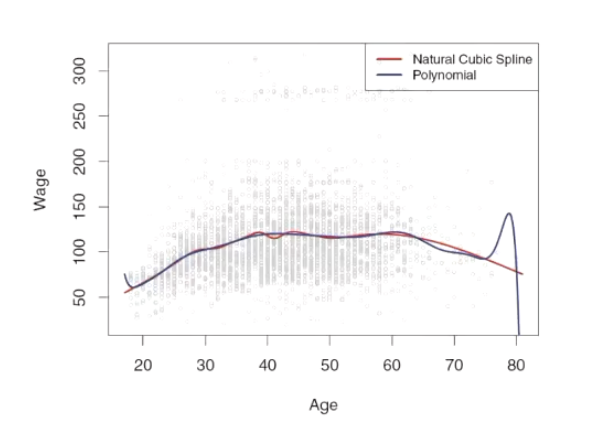
\includegraphics[width=0.6\textwidth]{polynomaol Vs natural cubic spline.png}
\end{figure}


\subsection{Smoothing splines}
\begin{itemize}
    \item In fitting a smooth curve to a dataset, we need to find some function $g(x)$ that can fit well to observed data. To achieve this goal we need to consider both adherence and smoothness.
    \item Adherence can be measured by the RSS, and the smoothness by $\int g''(t)^2 \; dt$. We construct the following objective function
    \begin{equation*}
        \sum_{i=1}^n (y_i - g(x_i))^2 + \lambda \int g''(t)^2 \;dt
    \end{equation*}
    where $\lambda$ is a non-negative tuning parameter, and the function g that minimising the equation is known as a smoothing spline.
    \item This equation can also be seen as "loss + penalty"
    \item when $\lambda = 0 $ the smoothness term has no effect, g will be very jumpy and will exactly interpolate the training observations
    \item when $\lambda \rightarrow \infty$ g will be perfectly smooth, i.e. the linear least squares line.
    \item $\lambda$ controls the bias-variance trade-off of the smoothing spline.
\end{itemize}

\subsubsection{The effective degrees of freedom}
\begin{itemize}
  \item A smoothing spline has far too many degrees of freedom, since placing a knot at each data point allows a great deal of flexibility. However, the tuning parameter $\lambda$ controls the smoothness of the spline, and hence the effective degrees of freedom.
  \item When $\lambda$ increases from $0$ to $\infty$, the effective degrees of freedom, denoted by $df_{\lambda}$, decrease from $n$ to $2$.
  \item $df_{\lambda}$ is a measure of the flexibility of the smoothing spline.


    \item Let $\hat y_{\lambda} = S_{\lambda}\,y$ denote the solution to (6), i.e.\ the $n$‐vector containing the fitted values of the smoothing spline at the training points $x_1,\dots,x_n$. Then
    \begin{equation*}
        df_{\lambda}\;=\;\sum_{i=1}^{n} \bigl\{S_{\lambda}\bigr\}_{ii},
    \end{equation*}
    i.e.\ the trace of the matrix~$S_{\lambda}$.
\end{itemize}
\subsubsection{Choosing the smoothing parameter $\lambda$}
\begin{itemize}
    \item For smoothing splines, there is no need to choose the number or location of the knots, as there is a knot at each training observation. Instead we need to choose the value of $\lambda$
    \item We can find the value of $\lambda$ that makes the CV RSS as small as possible. It turns out that the LOOCV can be computed very efficiently for smoothing splines, with essentially the same cost as computing a signly fit, using the formula;
    \begin{equation*}
        \mathrm{RSS}_{CV}(\lambda) = \sum_{i=1}^n [\frac{y_i - \hat{g}_\lambda(x_i)}{1 - {S_\lambda}_{ii}}]^2
    \end{equation*}
    This formula says that we can compute each of these leave-one-out fits using only $\hat{g}_\lambda$, the original fit to all of the data.
\end{itemize}

\subsubsection{ Smoothing Splines in R}
\begin{lstlisting}
# 5a. Fix degrees of freedom (df = roughness penalty lambda solves df)
fit_ss16 <- smooth.spline(x = age, y = wage, df = 16)

# 5b. Choose lambda by cross validation
fit_ssCV <- smooth.spline(x = age, y = wage, cv = TRUE)
fit_ssCV$df  # effective df chosen by CV
\end{lstlisting}


\subsection{Logical regression overview}
\begin{itemize}
    \item Local regression fits curves and surfaces to data by smoothing: the fit at $x_0$ is the value of a parametric function fitted only to those observation in a neighbourhood of $x_0$
    \item Local regression at $X = x_0$
    \begin{itemize}
        \item Gather the fraction  $s = k/n $ of training points whose $x_i$ are closest to $x_0$
        \item Assign a weight of $K_{i0} = \omega (\frac{x_i - x_0}{h(x_0)}$ to each point in this neighbourhood, where $h(x_0)$ is the bandwidth distance from $x_0$ to its kth closest $x_i$
        \item For a weighted least squares regression of the $y_i$ on the $x_i$ using the aforementioned weights, by finding $\hat{\beta}_0$ and $\hat{\beta}_1$ that minimise
        \begin{equation*}
            \sum_{i=1}^n K_{i0} (y_i - \beta_0 - \beta_1 x_i)^2
        \end{equation*}
        \item The fitted equation at $x_0$ is given by $\hat{f}(x_0) = \hat{\beta}_0 + \hat{\beta}_1 x_0$
    \end{itemize}
    \item We need to figure out how to define $\omega$
    \item Whether to fit a linear, constant or quadratic regression in step 3
    \item How to select an optimal span value s.
    \begin{itemize}
        \item s controls the \textbf{flexibility of the non-linear fit}. The smaller the value of s, the more local and wiggly will be our fit. Large s leads to a global fit to the data using all of the training observations. (can use CV to choose s)
    \end{itemize}
\end{itemize}

\subsubsection{Why local regression}
\begin{itemize}
        \item Adapts well to bias problems at boundaries and in regions of high curvature
        \item Easy to understand and interpret
        \item Methods have been developed that provide fast computation for one or more independant values
        \item Due to its simplicity, it can be tailored to work for many different distributional assumptions
        \item Having a local model enables derivation of response adaptive methods for span value and polynomial order selection in a straightforward manner
\end{itemize}

\subsubsection{How to choose the weight function $\omega(u)$}
\begin{itemize}
    \item We usually want a $\omega(u)$ function that peaks at $u = 0$ and decay smoothly to 0 as $u$ increases.
    \item We want a weight function that is non-zero only on a bounded interval rather than approaches zero when $u$ increases. This helps to increase computational speed
    \begin{equation*}
        \omega(u) = \begin{cases}
            (1 - |u|^3)^3 & |u| < 1\\
            0 & |u| \geq 1
        \end{cases}
    \end{equation*}
\end{itemize}


\subsubsection{How to choose the polynomial degree?}
\begin{itemize}
    \item A higher degree will produce a less biased, but more variable estimate
    \item Degree zero, or locally constant fitting, AKA moving average (quite simple)
    \item Degree greater than zero we increase bandwidth by a large amount without introducing intolerable bias
    \item Local quadratic fits better when there is a rapid change in slope
\end{itemize}


\subsection{Generalised linear models}
\begin{itemize}
    \item GLMs are a rich class of statistical methods which generalise the ordinary linear models in two directions
    \item \textit{Probability distribution}: instead of normal distribution, GLMs work with a general class of distributions, e.g. Poisson, Binom, and gamma
    \item \textit{Model for the mean:} in linear models the mean is a linear function of the predictors, \textbf{X}
    \begin{equation*}
        E[Y] = f(X)
    \end{equation*}
    In GLMs some smooth monotonic transformation of the mean is a linear function of X, with the linear and multiplicative models as special cases
    \begin{equation*}
        g(E[y]) = f(X)
    \end{equation*}
\end{itemize}

\subsubsection{Exponential family and the link function}
\begin{itemize}
    \item GLMs involve distributions that can be expressed in exponential form. When expressed in this form, there is a canonical parameter that is a function of the mean and a variance is also a function of the mean
    \begin{equation*}
        f(y|\theta,\phi) = e^{\frac{y \theta - b(\theta)}{\phi} + c(y,\theta)}
    \end{equation*}
    where $\theta$ is the canonical parameter and $\phi$ is the dispersion parameter that plays a role in defining the variance of y
    \item The canonical parameter $\theta$ is a function of $\mu$, denoted by $\theta(\mu)$ which is called the canonical link function
    \item GLMS WILL NOT BE ASSESSED IN THIS SUBJECT
  \item Normal: $\displaystyle \theta(\mu) = \mu$
  \item Poisson: $\displaystyle \theta(\mu) = \ln(\mu)$
  \item Exponential, gamma: $\displaystyle \theta(\mu) = -\mu^{-1}$
  \item Categorical, binomial, multinomial: $\displaystyle \theta(\mu) = \ln\!\biggl(\frac{\mu}{1-\mu}\biggr)$
\end{itemize}



\subsection{Generalised additive models}
\begin{itemize}
    \item Lowkey just adding functions together that model different variables.
    \item Generalised additive models (GAMs) are generalisations of GLMs
    \item The difference, in short is we are using smoothing functions of our predictors which can take on many forms.
    \item We can assume that the observed values $y$ are assumed to be of some exponential family distribution, and $\mu$ is still related to the model predictors via a link function. The key difference is that in linear form, some predictors now incorporate smooth functions, represented as $f(x)$, and this will allow for nonlinear relationships between these predictors and replace the response variable $y$
    \begin{equation*}
        y_i = \beta_0 + f_1(x_{i1}) + f_2(x_{i2}) + ... + f_p(x_{ip}) + \epsilon_i
    \end{equation*}
\end{itemize}

\begin{figure}[h!]
    \centering
    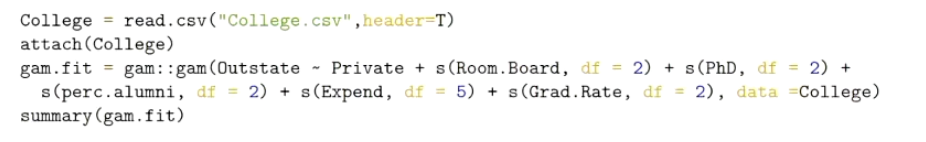
\includegraphics[width=0.6\textwidth]{GAM.png}
\end{figure}

\begin{itemize}
    \item In the image we have 6 predictors, Private is linear, the rest are non-linear. We assume non-linearity is not very high
    \item We look at df, they're all 1 hence not very significant. Only expand has 4 df hence quite significant. non-linear relationship is only significant for expend predictor.
\end{itemize}

\subsubsection{Fitting a GAM in R}
\begin{lstlisting}
# 1. Load package
library(gam)

# 2. Fit the full GAM with smoothing splines in year (4 df) and age (5 df)
gam_full <- gam(
  wage ~ s(year, df = 4)
       + s(age,  df = 5)
       + education,
  data   = Wage,
  family = gaussian
)

# 3. Plot each smooth term with 95% CI
par(mfrow = c(1, 2))
plot(gam_full, se = TRUE, col = "blue")

# 4. Test whether year needs to be nonlinear
gam_lin <- gam(
  wage ~ year
       + s(age, df = 5)
       + education,
  data   = Wage
)
anova(gam_lin, gam_full, test = "F")

# 5. Examine term significance & edf
summary(gam_full)

# 6. (Bonus) Logistic GAM for P(wage>250)
gam_bin <- gam(
  I(wage > 250) ~ s(age, df = 5)
               + education,
  family = binomial,
  data   = Wage
)
plot(gam_bin, se = TRUE)
\end{lstlisting}

\subsubsection{Pros and Cons of GAMs}

\begin{itemize}
  \item \textbf{Advantages of GAMs:}
    \begin{itemize}
      \item GAMs allow us to fit a non‐linear \(f_j\) to each \(X_j\), so that we can automatically model non‐linear relationships that standard linear regression will miss. This means that we don’t need to manually try out many different transformations on each variable individually.
      \item The non‐linear fits can potentially make more accurate predictions for the response \(Y\).
      \item Because the model is additive, we can still examine the effect of each \(X_j\) on \(Y\) individually while holding all of the other variables fixed. Hence, if we are interested in inference, GAMs provide a useful representation.
      \item The smoothness of the function \(f_j\) for the variable \(X_j\) can be summarised via degrees of freedom.
    \end{itemize}

  \item \textbf{Main limitation of GAMs:}
    \begin{itemize}
      \item The model is restricted to be additive. With many variables, \textbf{important interactions can be missed}. However, as with linear regression, we can manually add interaction terms to the GAM by including predictors of the form \(X_j \times X_k\). In addition, one can add low‐dimensional interaction functions \(f_{jk}(X_j, X_k)\) into the model; such terms can be fit using two‐dimensional smoothers (e.g.\ local regression) or two‐dimensional splines (not covered here).
    \end{itemize}
\end{itemize}

\newpage

\begin{center}
    \Large{Chapter 8: Tree Based methods}
\end{center}

\section{Chapter 8}
\begin{itemize}
    \item Trees cover classification and regression problems.
    \item These involves stratifying or segmenting the predictor space into a number of simple regions
    \item To make a prediction for a given observation, we typically use the mean or the mode of the training observations in the region to which it belongs.
    \item Since the set of splitting rules used to segment the predictor space can be summarised in a tree, these types of approaches are known as \textit{decision tree} methods.
    \item They are simple and useful for interpretation, but are not competitive with the best supervised learning approaches in terms of accuracy. 
\end{itemize}


\subsection{Regression Trees}

\begin{figure}[h!]
    \centering
    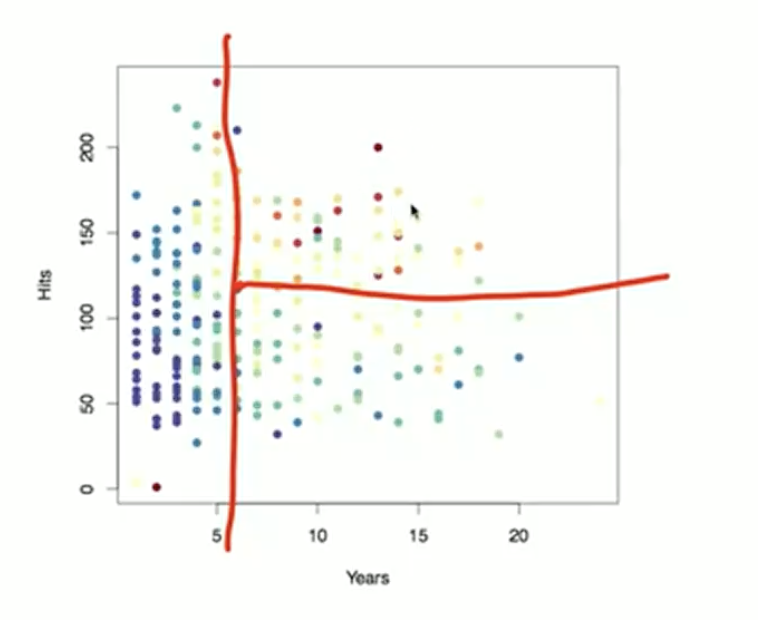
\includegraphics[width=0.6\textwidth]{scatter tree.png}
\end{figure}


\begin{figure}[h!]
    \centering
    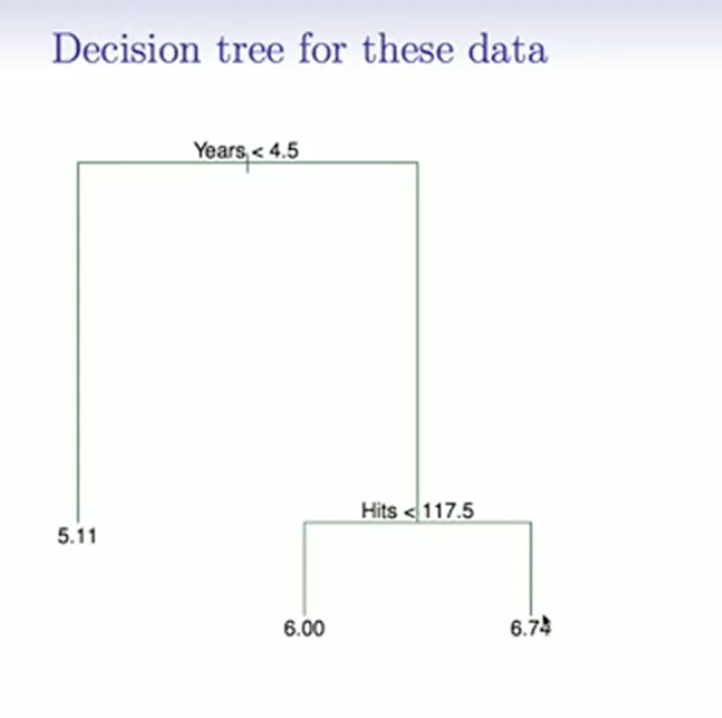
\includegraphics[width=0.6\textwidth]{simple tree.png}
\end{figure}

\subsubsection{Interpretation}
\begin{itemize}
    \item We are also saying, that number of hits is only for those with more than 4,5 years of experience.
\end{itemize}


\subsubsection{Terminology for trees}
\begin{itemize}
    \item $R_1, R_2$ and $R_3$ are known as terminal nodes
    \item The points along the tree where the predictor space is split are reffered to as internal nodes
    \item In the tree above: two internal nodes - Years<4.5 and Hits < 117.5
\end{itemize}


\subsubsection{Details of tree-building}
\begin{itemize}
    \item We divide the predictor space - the set of possible values for $X_1, X_2, ..., X_p$ into J distinct and non-overlapping regions $R_1, R_2, ..., R_J$
    \item For every observation that falls into the region $R_j$, we make the same prediction, which is simply the mean of the response values for the training observations in $R_J$
    \item We divide the predictor space into high-dimensional rectangles, or boxes, for simplicity and for ease of interpretation of the resulting predictive model.
    \item The goal is to find boxes $R_1, ..., R_J$ that minimize the RSS given by:
    \begin{equation*}
        \sum_{j=1}^J \sum_{i\in R_j} (y_i - \hat{y}_{R_j})^2
    \end{equation*}
    where $\hat{y}_{R_J}$ is the mean response for the training observations within the jth box.
    \item With this being said, it is unfeasible to consider each partition.
    \item For this reason we take a \textbf{\textit{top-down, greedy}} approach that is known as recursive binary splitting.
    \item It is \textbf{top-down} since it begins at the top and splits the predictor space into two new branches.
    \item IT is \textbf{greedy} because at each step of the tree-building process, the best split is made for the particular step, rather than looking ahead and picking a split that will lead to a better tree in some future step.
\end{itemize}


\subsubsection{Predictions for Trees}
\begin{itemize}
    \item We predict the response for a given test observation using the mean of the training observations in the region to which that test observation belongs.
\end{itemize}


\subsubsection{Pruning a tree}
\begin{itemize}
    \item If we create a massive tree, we will over-fit the data 
    \item A smaller tree with fewer splits might lead to a lower variance and better interpretation at the cost of a little bias.
    \item the best way is to create a large tree $T_0$ and then prune it back in order to obtain a \textbf{\textit{subtree}}
    \item Cost complexity pruning - aka weakest link pruning is used to do this
    \begin{equation*}
        \sum_{m=1}^{|T|} \sum_{i\in R_m} (y_i - \hat{y}_{R_m})^2 + \alpha |T|
    \end{equation*}
    $|T|$ denotes the number of terminal number of the tree $T$, $R_m$ is the rectangle corresponding to the $m$th terminal node, and $\hat{y}_{R_m}$ is the mean of the training observations in $R_m$
\end{itemize}

\subsubsection{Summary: tree algorithm}
\begin{itemize}
    \item Use recursive binary splitting to grow a large tree on the training data, stopping only when each terminal node has fewer than some minimum number of observations.
    \item Apply cost complexity pruning to the large tree in order to obtain a sequence of best subtrees, as a function of a.
    \item Use K-fold cross-validation to choose a. For each $k = 1,2,..., K$
    \begin{itemize}
        \item Repeat Steps 1 and 2 on the K-'th fraction of the training data, excluding the kth fold.
        \item Evaluate the mean squared prediction error on the data in the left-out kth fold, as a function of
    \end{itemize}
    Average the results, and pick $\alpha$ to minimise the average error
    \item Return the subtree from Step 2 that corresponds to the chosen value of $\alpha$
\end{itemize}

\subsubsection{Determining $\alpha$}
\begin{itemize}
    \item The size of $\alpha$ corresponds to the tree size. If $\alpha = 0$ then there is no penalty to tree size, so we get the largest tree that we fit.
    \item Hence as we increase $\alpha$ it puts more and more pressure on tree size so eventually we are forced to no splits
\end{itemize}

\begin{figure}[h!]
    \centering
    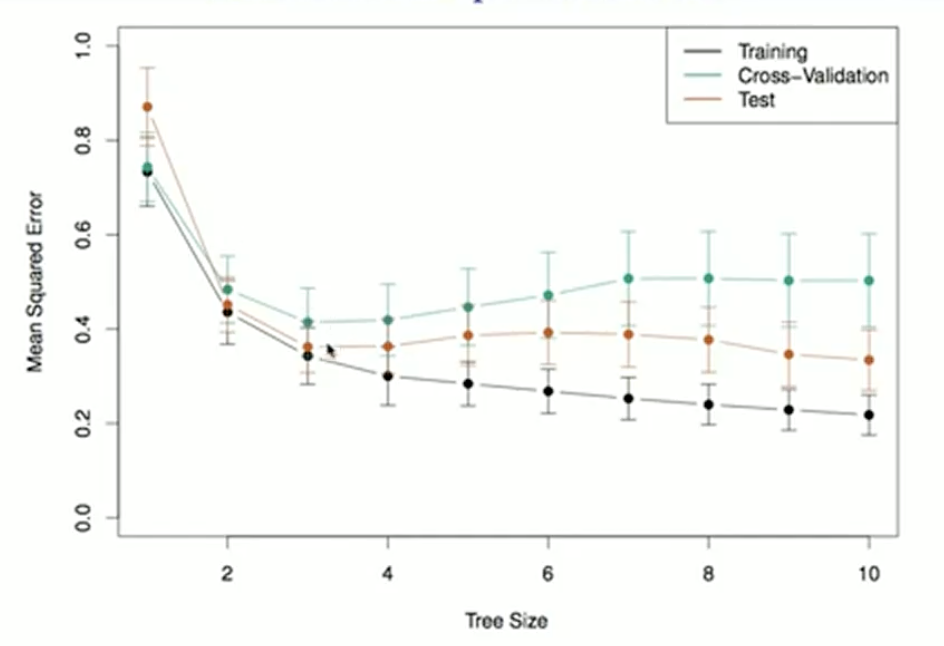
\includegraphics[width=0.6\textwidth]{tree size vs MSE.png}
\end{figure}


\subsubsection{Regression trees in R}

\begin{lstlisting}
library(MASS)
set.seed(1)
train = sample(1:nrow(Boston), nrow(Boston)/2)
tree.boston=tree(medv~.,Boston,subset=train)
summary(tree.boston)
plot(tree.boston)
text(tree.boston,pretty=0)
cv.boston=cv.tree(tree.boston)
plot(cv.boston$size,cv.boston$dev,type='b')
prune.boston=prune.tree(tree.boston,best=5)
plot(prune.boston)
text(prune.boston,pretty=0)
yhat=predict(tree.boston,newdata=Boston[-train,])
boston.test=Boston[-train,"medv"] #response in test set
plot(yhat,boston.test)
abline(0,1)
mean((yhat-boston.test)^2)
\end{lstlisting}

\subsection{Classification Trees}
\begin{itemize}
    \item Very similar to regression tree however we predict a qualitative response rather than quantitative.
    \item For a classification tree, we predict that each observation belongs to the most commonly occurring class of training observations.
    \item We again use recursive binary splitting to grow a classification tree.
    \item RSS cannot be found, hence we use classification error rate:
    \begin{equation*}
        E = 1  \max(\hat{p}_{mk})
    \end{equation*}
    where $\hat{p}_{mk}$ is the proportion of training observations in the $m$th region that are from the $k$th class.
\end{itemize}

\subsubsection{Gini index and Deviance}
\begin{itemize}
    \item The Gini Index is defined by
    \begin{equation*}
        G = \sum_{k=1}^K \hat{p}_{mk} (1 - \hat{p}_{mk})
    \end{equation*}
    a measure of total variance across the K classes. The Gini index takes on a small value if all of the $\hat{p}_{mk}$'s are close to zero or one.
    \item For this reason the Gini index is referred to as a measure of node purity - a small value indicates that a node contains predominantly observations from a single class.
    \item An altenitive to the Gini index is \textbf{cross-entropy}, given by 
    \begin{equation*}
        D = - \sum_{k=1}^K \hat{p}_{mk} \log(\hat{p}_{mk})
    \end{equation*}
    \item The \textbf{Gini index} and \textbf{cross-entropy} are very similar numerically
\end{itemize}


\subsubsection{Advantages and disadvantages of trees}
\begin{itemize}
    \item + Trees are very easy to explain to people. In fact, they are even easier to explain than linear regression
    \item + Some people believe that decision trees more closely mirror human decision-making than do the regression and classification approaches seen in previous units
    \item + Trees can be displayed graphically, and are easily interpreted even by a non-expert (especially if they are small)
    \item Trees can easily handle qualitative predictors without the need to create dummy variables
    \item - Unfortunately, trees generally do not have the same level of predictive accuracy as some of the other regression and classification approaches discussed in this subject.
    \item - Additionally, trees can be very non-robust. In other words, a small change in the data can cause a large change in the final estimated tree.
\end{itemize}


\subsubsection{Classification trees in R}
\begin{lstlisting}
library(tree)
library(ISLR)
names(Carseats)
attach(Carseats)
hist(Sales)
High=ifelse(Carseats$Sales<=8,"No","Yes") #Create variable "High"
High=as.factor(High) #Some version may not set High as factor properly
Carseats_new=data.frame(Carseats,High) #Merge "High" with "Carseats"
tree.carseats=tree(High~.-Sales, data=Carseats_new) #get rid of sales since High was made based on Sales
summary(tree.carseats)
plot(tree.carseats)
text(tree.carseats,pretty=0, cex = 0.7)

#Training correct prediction rate
tree.pred=predict(tree.carseats,Carseats_new,type="class")
table(tree.pred,Carseats_new$High)
mean(tree.pred==Carseats_new$High)

plot(tree.carseats)
text(tree.carseats,pretty=1)

#If pretty = 0 then the level names of a factor split attributes are 
#used unchanged. If pretty = NULL, the levels are presented by a, b, . z, 
#0 . 5. If pretty is a positive integer, abbreviate is applied to the 
#labels with that value for its argument.

tree.carseats

set.seed(2)
train=sample(1:nrow(Carseats_new), 200) #training subset
Carseats.test=Carseats_new[-train,] #test subset
High.test=High[-train]
tree.carseats=tree(High~.-Sales,Carseats_new,subset=train)
tree.pred=predict(tree.carseats,Carseats.test,type="class")
table(tree.pred,High.test)
mean(tree.pred==High.test) #1-test error rate

set.seed(3)
#FUN=prune.misclass uses classification error rate to guide the CV
cv.carseats=cv.tree(tree.carseats,FUN=prune.misclass)
names(cv.carseats)
cv.carseats
plot(cv.carseats$size,cv.carseats$dev,type="b")

prune.carseats=prune.misclass(tree.carseats,best=8) #from cv.carseats we see that the jump is at 8
plot(prune.carseats)
text(prune.carseats,pretty=0)
tree.pred=predict(prune.carseats,Carseats.test,type="class")
table(tree.pred,High.test)
mean(tree.pred==High.test)


#prune the tree by cost-complexity parameter alpha

prune.carseats1=prune.misclass(tree.carseats,k=3) #k=10 gives 2 nodes
summary(prune.carseats1)
plot(prune.carseats1)
text(prune.carseats1,pretty=1)
\end{lstlisting}



\newpage

\begin{center}
    \Large{Chapter 9: Support Vector Machines (SVM)}
\end{center}

\section{Chapter 9}

\begin{itemize}
    \item We attempt to approach the two-class classification problems in a direct way:
    \begin{itemize}
        \item \textbf{We try and find a plane that separates the classes in feature space}
    \end{itemize}
\end{itemize}

\subsection{Hyperplanes}

\subsubsection{What is a hyperplane?}
\begin{itemize}
    \item A hyperplane in p dimensions is a flat affine subspace of dimension p - 1
    \item In general the equation for a hyperplane has the form
    \begin{equation*}
        \beta_0 + \beta_1 X_1 + \beta_2 X_2 + ... + \beta_p X_p = 0
    \end{equation*}
    \item In $p = 2$ dimensions a hyperplane is a line.
    \item If $\beta_0 = 0$ the hyperplane goes through the origin, otherwise not.
    \item The vector $\beta = (\beta_1, \beta_2, ..., \beta_p)$ is called the normal vector - it points in a direction orthogonal to the surface of the hyperplane
\end{itemize}


\subsubsection{Hyperplane image:}
\begin{figure}[h!]
    \centering
    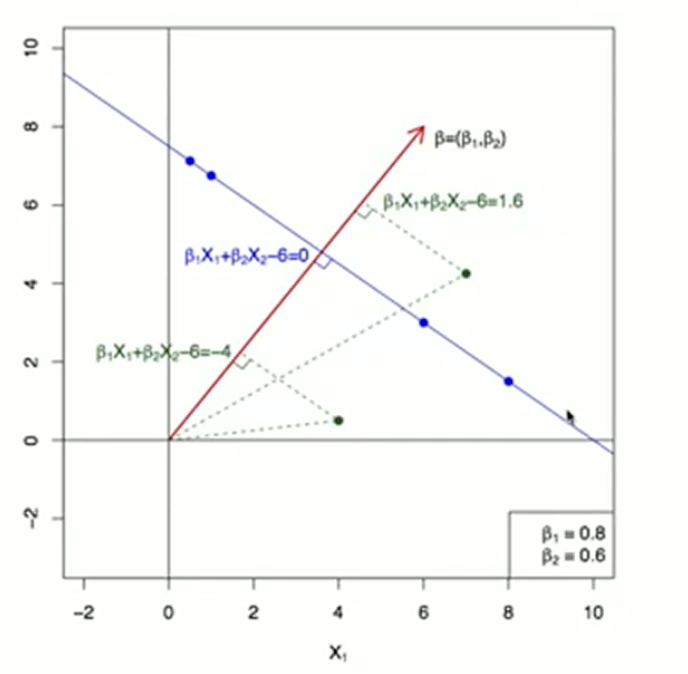
\includegraphics[width=0.6\textwidth]{hyperplane.png}
\end{figure}

\begin{itemize}
    \item Blue line is the hyperplane.
    \item Red line is orthogonal to the surface of the hyperplane.
    \item For any given point we can project it onto the normal (red line)
    \begin{itemize}
        \item From this we can get the distance from the origin to the point at which the random point projects.
    \end{itemize}
    \item Any point on the hyperplane has a function value of 0
    \item A special case in this image: the sum of squares of  $\beta_1$ and $\beta_2$ = 1, hence the direction vector is a unit vector, hence when you evaluate the function at any point, you get the euclidean distance.
    \item The value of the function is the distance from the hyperplane
\end{itemize}


\subsubsection{Separating Hyperplanes}

\begin{figure}[h!]
    \centering
    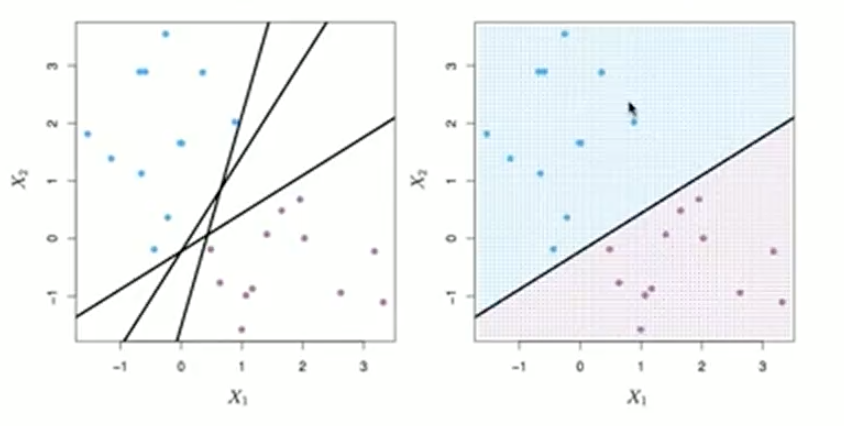
\includegraphics[width=0.6\textwidth]{Seperating hyperplanes.png}
\end{figure}
\begin{itemize}
    \item Technically all of the lines on the left separate the blue an red dots
    \item If; $f(x) = \beta_0 + \beta_1 X_1 + ... + \beta_p X_p$, then $f(X)>0$ points on one side of the hyperplane, and $f(X)<0$ for points on the other.
    \item We can code the coloured points as $Y_i = +1$ for blue, and $Y_i = -1$ for red, then if $Y_i f(X_i) > 0$ for all i, $f(X) = 0$ defines a separating hyperplane
\end{itemize}

\subsection{Maximal Margin Classifier}

\begin{figure}[h!]
    \centering
    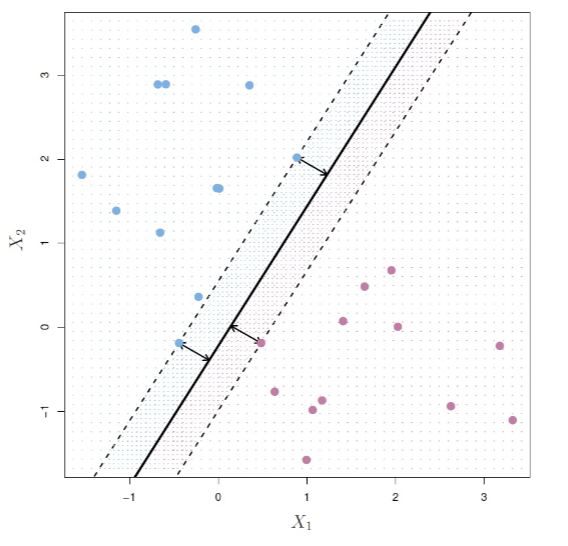
\includegraphics[width=0.6\textwidth]{Maximal margin classifier.png}
\end{figure}

\begin{itemize}
    \item Among all separating hyperplanes, find the one that makes the biggest gap or margin between the two classes
    \item The hyperplane shown is exactly equidistant from the closest blue point and the closest red point.
    \begin{itemize}
        \item The thought process is, if you make a big gap on the training data then you will hopefully classify the test data sufficiently - possibly overfitting.
    \end{itemize}
\end{itemize}

\subsubsection{Construction of the Maximal Margin classifier}

\begin{itemize}
    \item We wanted to Maximise M
    \item subject to $\sum_{j=1}^P \beta_j^2 = 1$
    \item Where $y_i (\beta_0 + \beta_1 x_{i1} + ... + \beta_p x_{ip}) \geq M$ for all $i = 1,..., N$
\end{itemize}

\begin{lstlisting}
svm() #solves this properly
\end{lstlisting}


\subsection{Support Vector Classifier}
\begin{itemize}
    \item Sometimes data is non-separable.
    \item Sometimes Data is noisy, where there is a single outlier that will change the hyperplane drastically. (Does not make sense to change the hyperplane by so much for a single point)
\end{itemize}

\begin{lstlisting}
library(e1071)
# Choices for kernel include "linear", "polynomial", "radial basis", and "sigmoid"
# cost: cost of constraints violation (default: 1)

svmfit.1 <- svm(y ~ ., data = dat, kernel = "linear",  cost = 10, scale = FALSE)
plot(svmfit.1, dat)

# The index of the resulting support vectors in the data matrix.
svmfit.1$index
summary(svmfit.1)

\end{lstlisting}

\begin{itemize}
    \item Cost is the emphasis on relation to fit.
    \item A large cost leads to a large emphasis to fit for the training data which decreases Bias increases Variance.
    \item A high Cost means the margin is very small hence less support vectors
    \item Lower cost means the margin is bigger, hence more support vectors.
~~\end{itemize}

\subsubsection{Soft margin}

\begin{itemize}
    \item A soft margin is a section of "leeway" that allows for points of the wrong side of the margin.
    \item They are used when data in inseparable.
    \item We want to maximise M subject to $\sum_{j=1}^p \beta_j^2 = 1$
    \item $y_i (\beta_0 + \beta_1 x_{i1} + \beta_2 x_{i2} + ... + \beta_p x_{ip}) \geq M(1 - \epsilon_i$) where $\epsilon_i \geq 0, \sum_{i=1}^n \epsilon_i \leq C$
    \item \textbf{$C$ is a regularisation parameter, that determines that determines the distance of the margin.} C is inversly related to cost.
    \item each $\epsilon_i$ is proportional to the distance from each point within the margin to the hyperplane. (there is an $\epsilon$ for each point)
    \item \textbf{Standardise all variables}
    \item There is a bias-variance trade-off
    \begin{itemize}
        \item When C is small, we seek narrow margins that are rarely violated; this amounts to a classifier that is highly fit to the data, which may have low bias but high variance.
        \item On the other hand, when C is larger, the margin is wider and we allow more violations to it; this amounts to fitting the data less hard and obtaining a classifier that is potentially more biased but may have lower variance.
    \end{itemize}
\end{itemize}

\subsection{Feature expansion}

\begin{itemize}
    \item We can now enlarge the feature space by including transformations; e.g. $X_1^2, X_1^3, X_1 X_2, X_2^2, ....$ Hence going from a $p$-dimensional space to a $M>p$ dimensional space.
    \item Fit a support-vector classifier in the enlarged space.
    \item This result in the non-linear decision boundaries n the original space
    \item Say we now use $(X_1, X_2, X_1^2, X_2^2, X_1 X_2)$ instead of just $(X_1, X_2)$. The decision boundary would be of the form
    \begin{equation*}
        \beta_0 + \beta_1 X_1 + \beta_2 X_2 + \beta_3 X^2_1 + \beta_4 X^2_2 + \beta_5 X_1 X_2 = 0
    \end{equation*}
    
\end{itemize}


\begin{figure}[h!]
    \centering
    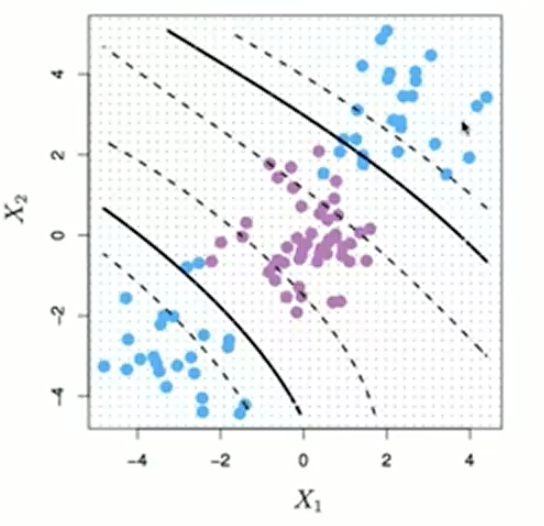
\includegraphics[width=0.6\textwidth]{bigger decision boundary.png}
\end{figure}



\subsection{Nonlinearities and Kernels}

\begin{itemize}
    \item Polynomials (especially high-demand ones) get wild rather fast.
    \item kernels are more elegant and controlled
\end{itemize}

\subsubsection{Inner products and support vectors}
\begin{itemize}
    \item $\langle x_i, x_{i'} \rangle = \sum_{j=1}^p x_{ij} x_{i'j}$ inner product between vectors
    \item The linear support vector classifier can be represented as 
    \begin{equation*}
        f(x) = \beta_0 + \sum_{i=1}^n \alpha_i \langle x, x_i \rangle \text{n parameters}
    \end{equation*}
    \item To estimate the paramters $\alpha_1, ..., \alpha_n$ and $\beta_0$, all we need are the $\binom{n}{2}$ inner products $\langle x_i, x_{i'} \rangle$ between all pairs of training observations.
    \item It turns out most $\hat{\alpha}$ can be 0
    \begin{equation*}
        f(x) = \beta_0 + \sum_{i\in S} \hat{\alpha}_i \langle x, x_i \rangle
    \end{equation*}
    \item S is the support set of indicies i such that $\hat{\alpha}_i > 0$
    \item Support vectors are the vectors within the boundaries set out in the support vector classifier, any value outside of the dotted lines, are no longer used to calculate the hyperplane, however those points were needed to know which points were significant. (all points outside have $\alpha = 0$)
\end{itemize}

\subsubsection{Kernels and Support Vector Machines}

\begin{itemize}
    \item If we can compute inner-products between observations, we can fit a SV classifier
    \item Some special kernel functions do this for us. e.g.
    \subitem Polynomial kernel function:
    \begin{equation*}
        K(x_i, x_{i'}) = (1 + \sum_{j=1}^p x_{ij}x_{i' j})^d
    \end{equation*}
    computes inner products for $d$ dimensional polynomials - $\binom{p + d}{d}$ basis functions
\end{itemize}

\pagebreak
\subsection{Radial Kernel}

\begin{equation*}
    K(x_i,x_{i'}) = \exp{(- \gamma\sum_{j=1}^p (x_ij} - x_{i'j})^2)
\end{equation*}



\begin{figure}[h!]
    \centering
    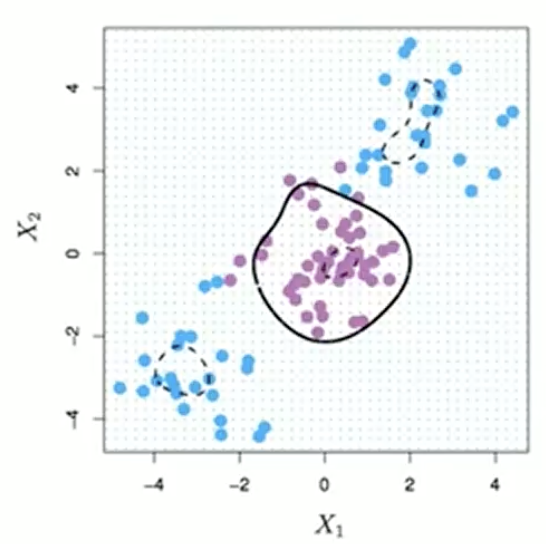
\includegraphics[width=0.6\textwidth]{Radial kernel.png}
\end{figure}


\begin{itemize}
    \item $f(x) = \beta_0 + \sum_{i\in S}\hat{\alpha}_i K(x,x_i)$
    \item Implicit feature space; very high dimensional
    \item Controls variance by squashing down most dimensions severely
\end{itemize}


\subsubsection{ROC curve}

\begin{itemize}
    \item The ROC curve us obtained by changing the threshold 0 to threshold t in $\hat{f}(X) > t$ and recording false positive and true positive rates as $t$ varies.
\end{itemize}



\subsection{SVM's with more than two classes}

\begin{itemize}
  \item \textbf{The One‐Versus‐One classification}
    \begin{itemize}
      \item Suppose that there are \(K > 2\) classes. A one‐versus‐one (or all‐pairs) approach constructs \(\binom{K}{2}\) SVMs, each of which compares a pair of classes.
      \item For example, one such SVM might compare the \(k\)th class (coded as \(+1\)) to the \(k'\)th class (coded as \(-1\)).
      \item We classify a test observation using each of the \(\binom{K}{2}\) classifiers, and we tally the number of times that the test observation is assigned to each of the \(K\) classes.
      \item The final classification is performed by assigning the test observation to the class to which it was most frequently assigned in these \(\binom{K}{2}\) pairwise classifications.
    \end{itemize}
    \item \textbf{The One‐Versus‐All classification}
    \begin{itemize}
        \item The one‐versus‐all approach is an alternative procedure for applying SVMs in the case of \(K > 2\) classes. We fit \(K\) SVMs, each time comparing one of the \(K\) classes to the remaining \(K-1\) classes.
        \item Let \(\beta_{0k}, \beta_{1k}, \dots, \beta_{pk}\) denote the parameters that result from fitting an SVM comparing the \(k\)th class (coded as \(+1\)) to the others (coded as \(-1\)).
        \item Let \(x^*\) denote a test observation. We assign the observation to the class for which
        \[
        \beta_{0k} \;+\; \beta_{1k}\,x^*_1 \;+\; \beta_{2k}\,x^*_2 \;+\; \cdots \;+\; \beta_{pk}\,x^*_p
        \]
    is largest, as this amounts to a high level of confidence that the test observation belongs to the \(k\)th class rather than to any of the other classes.
    \end{itemize}
\end{itemize}

\subsection{Pros Vs Cons of SVM}

\textbf{Pros:}
\begin{itemize}
  \item It works really well with a clear margin of separation.
  \item It is effective in high‐dimensional spaces.
  \item It only uses a subset of training points in the decision function (i.e., support vectors), so it is also memory‐efficient.
\end{itemize}

\noindent \textbf{Cons:}
\begin{itemize}
  \item It doesn’t perform well when we have a large data set because the required training time is higher.
  \item It also doesn’t perform very well when the data set has more noise, i.e., target classes are overlapping.
  \item SVM doesn’t directly provide probability estimates.
\end{itemize}


\pagebreak
\begin{center}
    \Large{Chapter 10: Unsupervised Learning}
\end{center}

\section{Chapter 10}

\begin{itemize}
    \item Unsupervised learning observes only the features $X_1, X_2, ..., X_p$. We are not interested in prediction, because we do not have an associated response variable Y.
\end{itemize}

\subsection{Goals/Challenges of Unsupervised learning}


\noindent\textbf{Goals}
\begin{itemize}
    \item The goal is to discover interesting things about the measurements: seeing whether there is an informative way to visualise the data, or whether there is subgroups among the data.
    \item There is two methods;
    \begin{itemize}
        \item \textbf{Principal components analysis} - a tool used for data visualisation or data pre-processing before supervised techniques are applied
        \item \textbf{Clustering} - a broad class of methods for discovering unknown subgroups
    \end{itemize}
    \item It is often easier to obtain unlabelled data - from a lab instrument or computer - than labelled data, which can require human intervention.
\end{itemize}


\noindent\textbf{Challenges}
\begin{itemize}
    \item It is more subjective than supervised learning as there is no simple goal for the analysis, such as prediction of a response
    \item However techniques for unsupervised learning are of growing importance.
\end{itemize}



\subsection{Principal Components Analysis (PCA)}

\begin{itemize}
    \item PCA produces a low-dimensional representation of a dataset. It finds a sequence of linear combinations of the variables that have maximal variance, and are mutually uncorrelated.
    \item Apart from producing derived variables for use in unsupervised learning problems, PCA also serves as a tool for data visualisation
\end{itemize}


\subsubsection{PCA analysis: details}
\begin{itemize}
    \item The first principal component of a set of features $X_1, X_2, ..., X_p$ is the normalised linear combination of the features
    \begin{equation*}
        Z_1 = \phi_{11}X_1 + \phi_{21} X_2 + ... + \phi_{p1} X_p
    \end{equation*}
    that has the largest variance. Normalised means that $\sum_{j=1}^p \phi_{j1}^2 = 1$
    \item The $\phi_11, ..., \phi_{p1}$ are hte loadings of the first principal component, making up a loading vector $\phi_1 = (\phi_{11} \; \phi_{21} \; ... \; \phi_{p1})^\top$
    \item The sum of squares for the loadings = 1
\end{itemize}

\subsubsection{Computation of Principal components}
\begin{itemize}
    \item Suppose there is a $n \text{x} p$ dataset $\mathbf{X}$. Since we only care about variance, we assume that each variable in $\mathbf{X}$ has been centred to have mean zero.
    \item We then look for the linear combination of the sample feature values in teh form
    \begin{equation*}
        z_{i1} = \phi_{11} x_{i1} + \phi_{21} x_{i2} + ... + \phi_{p1} x_{ip}
    \end{equation*}
    for $i = 1,...,n$ and $\sum_{j=1}^p \phi_{j1}^2 = 1$.
    \item Since each of the $x_{ij}$ has mean zero, then so does $z_{i1}$. Hence the sample variance of the $z_{i1}$ can be written as $\frac{1}{n}\sum_{i=1}^n z_{i1}^2$
    \item Plugging in the formula above to the first principal component loading vector solves the optimisation problem maximise$\frac{1}{n}\sum_{i=1}^n (\sum_{j=1}^p \phi_{j1} x_{ij})^2$ which si subject to $\sum_{j=1}^p \phi_{j1}^2 = 1$.
    \item We refer to $Z_1$ as the first principal component, with realized values $z_{11}, ..., z_{p1}$
\end{itemize}

\subsubsection{Geometry of PCA}
\begin{itemize}
    \item The loading vector $\phi_1$ with elements $\phi_{11}, \phi_{21}, ..., \phi_{p1}$ defines a direction in feature space align which the data vary most.
    \item If we project the $n$ data points $x_1, ..., x_n$ onto this direction, the projected values are the principal component scores $z_{11}, ...., z_{n1}$ themselves.
\end{itemize}

\begin{figure}[h!]
    \centering
    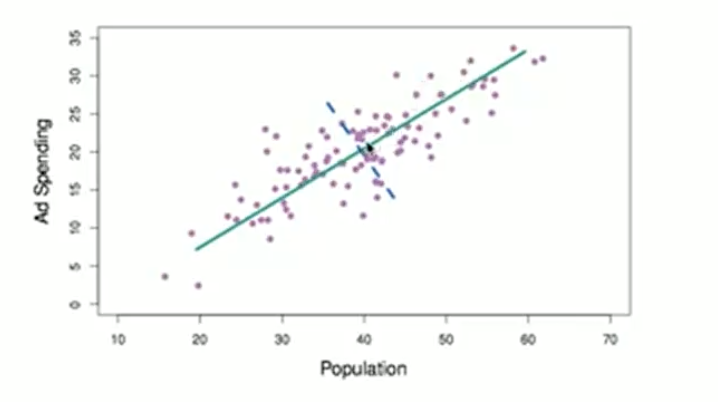
\includegraphics[width=0.6\textwidth]{PCA exmaple.png}
\end{figure}

\begin{itemize}
    \item In this example the first principal component is the solid line.
    \item The loading vector is the vector that starts in the middle to the top right.
    \item The computed values are the projection of each point onto the line
    \item For any values on the right of the dashed line, the $z$ will be positive, any on the left will be negative.
\end{itemize}



\subsubsection{Further principal components}
\begin{itemize}
    \item The second principal component $Z_2$ is teh linear combination of $X_1, ..., X_p$ that has maximal variance along all linear combinations that are uncorrelated with $Z_1$
    \item The second principal component scores $z_{12}, z_{22}, ..., z_{n2}$ take the form 
    \begin{equation*}
        z_{i2} = \phi_{12} x_{i1} + \phi_{22} x_{i2} + ... + \phi_{p2} x_{ip}
    \end{equation*}
    where $\phi_2$ is the second principal component loading vector, with elements $\phi_{12}, \phi_{22}, ..., \phi_{p2}$
\end{itemize}



\subsubsection{Scaling of variables}

\begin{itemize}
    \item Scaling is crucial, if variables are measured in different units, then it is impossible for the PCA to determine the difference of variables
\end{itemize}

\subsubsection{Proportion Variance explained (PVE)}

\begin{itemize}
    \item To understand the strength of each component we are interested in knowing the proportion of variance explained by each one
    \item The total variance present in a data set  is defined as
    \begin{equation*}
        \sum_{j=1}^p \text{Var}(X_j) = \sum_{j=1}^p \frac{1}{n} \sum_{i=1}^n x^2_{ij}
    \end{equation*}
    and the variance is explained by the $m$th principal component is Var$(Z_m) = \frac{1}{n} \sum_{i=1}^n z_{im}^2$
    \item It can be shown that $\sum_{j=1}^p \text{Var}(X_j) = \sum_{m=1}^M \text{Var}(Z_m)$ with $M = \min(n-1, p)$
    \item Hence the PVE of $Z_m$ is given by
    \begin{equation*}
        \frac{\sum_{i=1}^n z_{im}^2}{\sum_{j=1}^p\sum_{i=1}^n x_{ij}^2}
    \end{equation*}
    \item The PVEs sum to one.
\end{itemize}


\subsection{PCA in R}

\begin{lstlisting}
states=row.names(USArrests)
states
names(USArrests)
apply(USArrests, 2, mean) #2 for columns
apply(USArrests, 2, var) #2 for columns
pr.out=prcomp(USArrests, scale=TRUE) #PCA with standardisation
names(pr.out)
pr.out$center # mean of original columns
pr.out$scale # s.d. of original columns
pr.out$rotation # PC loading vectors
dim(pr.out$x) # PC scores, i.e. transformed features
biplot(pr.out, scale=0)

#PVE
pr.var=pr.out$sdev^2 #variance of PCs
pr.var
pve=pr.var/sum(pr.var) #calculating PVE (proportion of var explained)
pve

plot(pve, xlab="Principal Component", ylab="Proportion of Variance Explained", 
     ylim=c(0,1),type='b')
plot(cumsum(pve), xlab="Principal Component", ylab="Cumulative Proportion of Variance Explained", 
     ylim=c(0,1),type='b') #cumsum() calculates cumulative sum of elements

\end{lstlisting}

\subsection{Clustering methods}

\begin{itemize}
    \item Clustering refers to a very broad set of techniques for finding subgroups, or clusters in a data set.
    \item We seek a partition of the data into distinct groups so that the observations within each group are quite similar to each other.
    \item We must define what it means to make two or more observations to be similar or different.
\end{itemize}

\subsubsection{PCA vs Clustering}
\begin{itemize}
    \item PCA looks for a low-dimensional representation of the observations that explains a good fraction of the variance
    \item Clustering looks for homogeneous subgroups among the observations.
\end{itemize}


\subsubsection{K-means clustering}

\begin{itemize}
    \item For a predetermines K, K-means clustering will split the given data into K groups
\end{itemize}

\noindent\textbf{Details}

\begin{itemize}
    \item Let $C_1, ..., C_k$ denote the indices of the observations in each cluster. These sets satisfy two properties:
    \begin{enumerate}
        \item $C_1 \cup C_2 \cup ... \cup C_k = \{1,...,n\}$. meaning each observation belongs to at least one of the K clusters.
        \item $C_k \cap C_{k'} = \emptyset$ for all $k \neq k'$. Meaning the clusters are non-overlapping: no observation belongs to more than one cluster.
    \end{enumerate}
    \item The idea behind K-means clustering is that a good clustering is one for which the within-cluster variation is as small as possible.
    \item The within-cluster variation for cluster $C_k$ is a measure WCV($C_k$) of the amount by which the observations within a cluster differ from each other.
    \item Hence we want to solve;
    \begin{equation*}
        \text{minimise}\{\sum_{k=1}^K \text{WCV}(C_k)\}
    \end{equation*}
    \item In words - we want to partition the observations into K clusters such that the total within-cluster variation, summed over all KK clusters is as small as possible.
\end{itemize}



\noindent \textbf{Within cluster variation}

\begin{itemize}
    \item WCV($C_k$) is defined as
    \begin{equation*}
        \text{WCV}(C_k) = \frac{1}{|C_k|}\sum_{i, i' \in C_k} \sum_{j=1}^p (x_{ij} - x_{i'j})^2 = 2 \cdot \sum_{i, i' \in C_k} \sum_{j=1}^p (c_{ij} - \bar{x}_{kj})^2
    \end{equation*}
    where $|C_k|$ denotes the number of observations in the $k$th cluster. and $\bar{x}_{ij}$ is the mean for feature $j$ in cluster $C_k$
    \item Hence we want to minimise:
    \begin{equation*}
        \sum_{k=1}^K \frac{1}{|C_k|}\sum_{i, i' \in C_k} \sum_{j=1}^p (x_{ij} - x_{i'j})^2
    \end{equation*}
\end{itemize}


\subsubsection{K-means Clustering Algorithm}

\begin{itemize}
  \item[1.] Randomly assign a number, from $1$ to $K$, to each of the observations.  These serve as initial cluster assignments for the observations, denoted by 
  \[
    C_{1}^{(1)},\,C_{2}^{(1)},\dots,C_{K}^{(1)}.
  \]
  Let $\ell = 1$.
  
  \item[2.] 
    \begin{itemize}
      \item[(a)] For each $k = 1,\dots,K$, let $C_{k}^{(\ell)}$ be the current cluster.  Compute its centroid
      \[
        \bigl(\,\bar{x}_{k1}^{(\ell)},\,\bar{x}_{k2}^{(\ell)},\,\dots,\,\bar{x}_{kp}^{(\ell)}\bigr),
      \]
      i.e.\ the vector of the $p$ feature means for the observations in $C_{k}^{(\ell)}$.
      
      \item[(b)] Assign each observation to the cluster whose centroid is closest (where “closest” is defined using Euclidean distance), thereby generating new clusters 
      \[
        C_{1}^{(\ell+1)},\,C_{2}^{(\ell+1)},\,\dots,\,C_{K}^{(\ell+1)}.
      \]
      If 
      \[
        C_{1}^{(\ell+1)},\,C_{2}^{(\ell+1)},\,\dots,\,C_{K}^{(\ell+1)}
        \;\text{are different from}\;
        C_{1}^{(\ell)},\,C_{2}^{(\ell)},\,\dots,\,C_{K}^{(\ell)},
      \]
      then let $\ell \leftarrow \ell + 1$ and repeat Step 2; otherwise, return 
      \[
        C_{1}^{(\ell)},\,C_{2}^{(\ell)},\,\dots,\,C_{K}^{(\ell)}
      \]
      as the final output.
    \end{itemize}
\end{itemize}


\begin{figure}[h!]
    \centering
    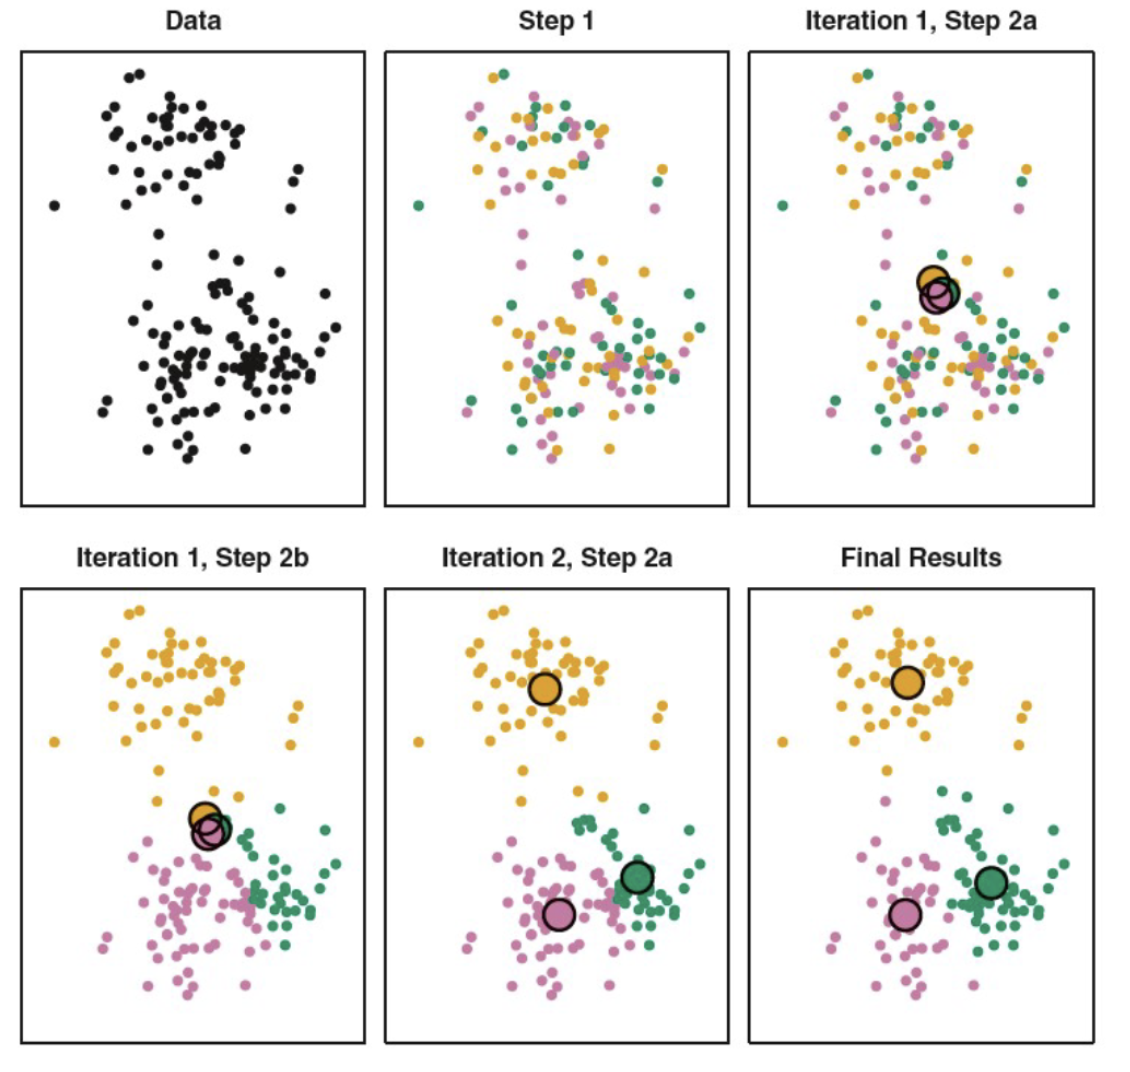
\includegraphics[width=0.5\textwidth]{K means clustering.png}
\end{figure}


\begin{itemize}
    \item Depending on where we start the algorithm, changes the actual clusters:
\end{itemize}

\begin{figure}[h!]
    \centering
    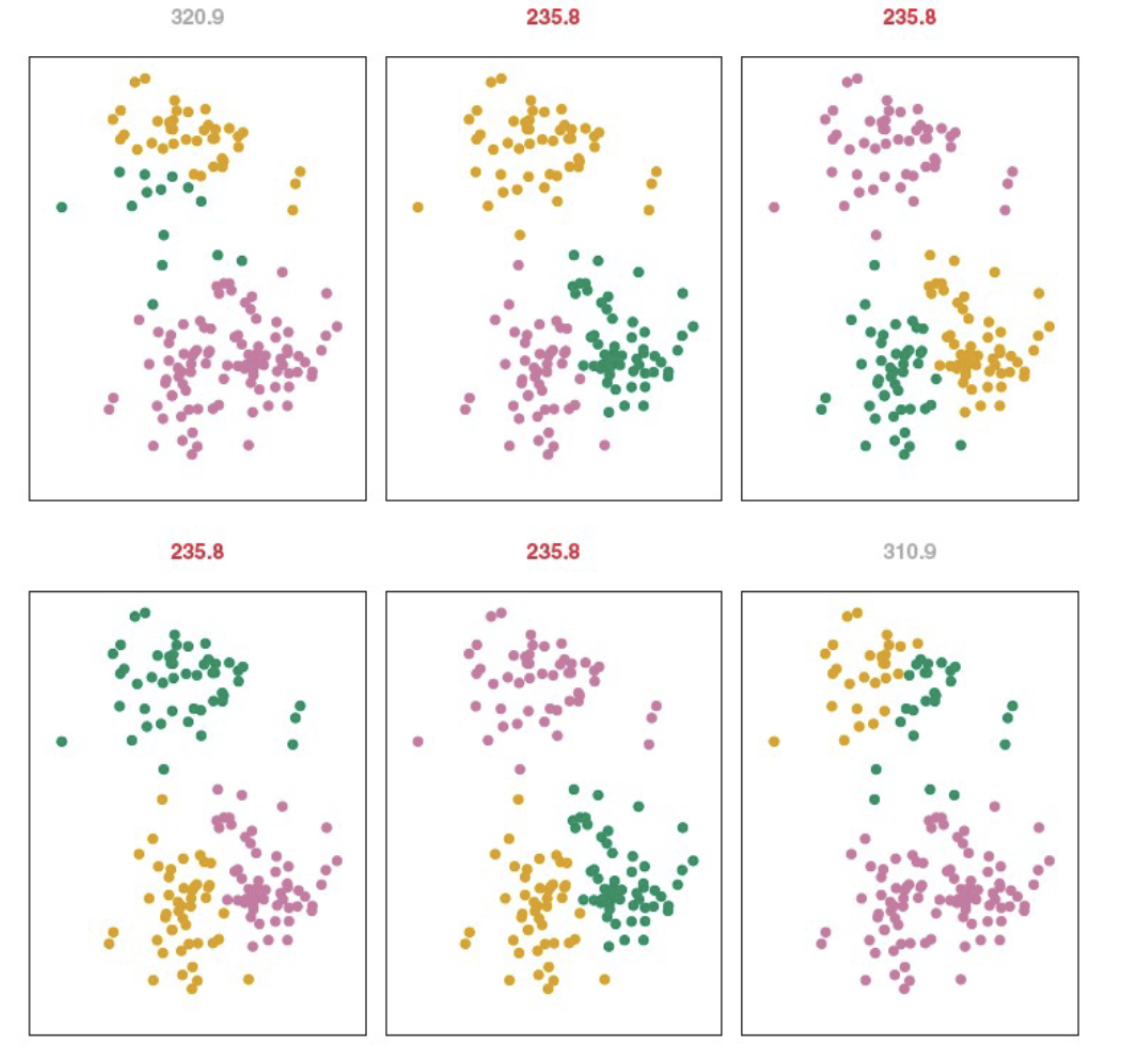
\includegraphics[width=0.5\textwidth]{K means clustering 2.png}
\end{figure}


\subsubsection{K-means clustering in R}

\begin{lstlisting}
set.seed(2)
x=matrix(rnorm(100*2),ncol = 2)
x
plot(x)
x[1:25,1]=x[1:25,1]+3
x[1:25,2]=x[1:25,2]-4
#Only changed the first 25 rows
x
plot(x)
km.out=kmeans(x,2,nstart=20) #20 random sets were chosen and report the best one
km.out$cluster #shows the distribution of each point to a cluster
plot(x, col=(km.out$cluster+1), main="K-Means Clustering Results with K=2", 
     xlab="", ylab="", pch=20, cex=2)
#Change K for the amount of cluster we want (K = 2 in this case)
\end{lstlisting}


\subsection{Hierarchical Clustering}

\begin{itemize}
    \item K-means clustering requires us to pre-specify the number of clusters K. This can be a disadvantage
    \item Hierarchical clustering is an alternative approach which does not require that we commit to a particular choice of K.
\end{itemize}

\begin{figure}[h!]
    \centering
    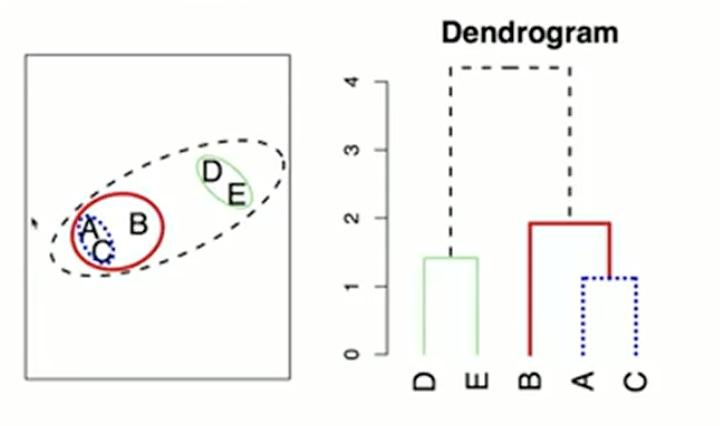
\includegraphics[width=0.5\textwidth]{heirachal cluster.png}
\end{figure}

\begin{figure}[h!]
    \centering
    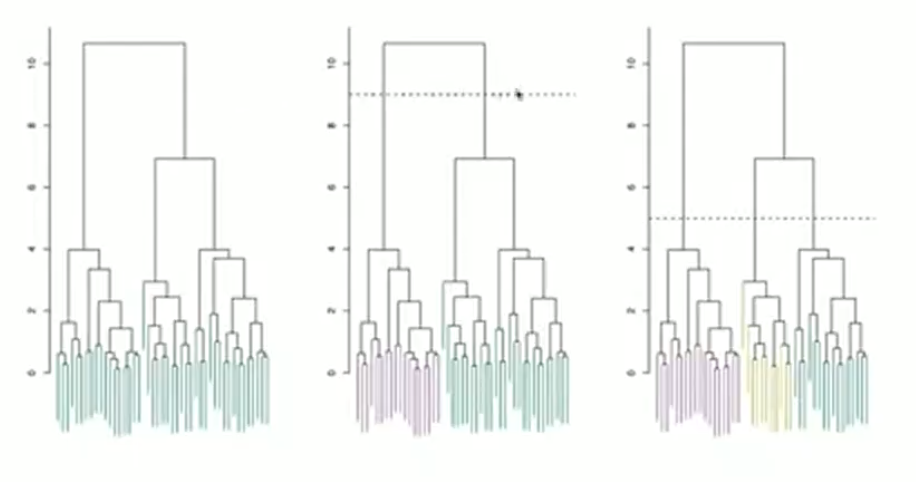
\includegraphics[width=0.5\textwidth]{Heirarchical clustering Image.png}
\end{figure}

\begin{itemize}
    \item As show, depending on the cut-off, depends on the Split of the data.
    \item Hierarchical clustering works bottom up, joining the two closest points/clusters at each step and repeats until all clusters are as one.
\end{itemize}

\subsubsection{Linkage types}
\begin{itemize}
  \item \textbf{Complete:} Maximal inter‐cluster dissimilarity. Compute all pairwise dissimilarities between the observations in cluster A and the observations in cluster B, and record the \emph{largest} of these dissimilarities.
  \begin{itemize}
      \item Looking for the largest distance points from each cluster.
  \end{itemize}
  \item \textbf{Single:} Minimal inter‐cluster dissimilarity. Compute all pairwise dissimilarities between the observations in cluster A and the observations in cluster B, and record the \emph{smallest} of these dissimilarities.
  \begin{itemize}
      \item Find the smallest distance points from each cluster
  \end{itemize}
  \item \textbf{Average:} Mean inter‐cluster dissimilarity. Compute all pairwise dissimilarities between the observations in cluster A and the observations in cluster B, and record the \emph{average} of these dissimilarities.
  \begin{itemize}
      \item Average of distances between all points in each cluster
  \end{itemize}
  \item \textbf{Centroid:} Dissimilarity between the centroid for cluster A (a mean vector of length $p$) and the centroid for cluster B. Centroid linkage can result in undesirable \emph{inversions}.
  \begin{itemize}
      \item Take Centroid/average of each cluster and find the distance.
  \end{itemize}
\end{itemize}


\subsubsection{Choice of Dissimilarity Measure}

\begin{itemize}
    \item We have used Euclidean distance as the dissimilarity measure. But sometimes other dissimilarity measures might be preferred.
    \item For example, correlation-based distance considers two observations to be similar if their features are highly correlated, even though the observed values may be far apart in terms of Euclidean distance. Correlation-based distance focuses on the shapes of observation profiles rather than their magnitudes.
    \item The choice of dissimilarity measure is very important, as it has a strong effect on the resulting dendrogram. In general, careful attention should be paid to the type of data being clustered and the scientific question at hand. These considerations should determine what type of dissimilarity measure is used for hierarchical clustering.
\end{itemize}



\subsubsection{Hierarchical clustering in R}


\begin{itemize}
    \item When plotting we are looking for the most symmetrical tree
\end{itemize}
\begin{lstlisting}
#x defined in K-means clustering
#create the clusters
hc.complete=hclust(dist(x), method="complete") #complete
hc.average=hclust(dist(x), method="average") #average
hc.single=hclust(dist(x), method="single") #single

#Plot the clustering
plot(hc.complete,main="Complete Linkage", xlab="", sub="", cex=.9)
plot(hc.average, main="Average Linkage", xlab="", sub="", cex=.9)
plot(hc.single, main="Single Linkage", xlab="", sub="", cex=.9)

#Cut the trees
cutree(hc.complete, 5) #number refers to amount of clusters. NOT HEIGHT
cutree(hc.average, 2)
cutree(hc.single, 2)


xsc=scale(x) #Scaling the variables beforehand

plot(hclust(dist(xsc), method="complete"), 
     main="Hierarchical Clustering with Scaled Features")

x=matrix(rnorm(30*3), ncol=3)
dd=as.dist(1-cor(t(x))) # use 1-correlation as the distance function
plot(hclust(dd, method="complete"), 
     main="Complete Linkage with Correlation-Based Distance", xlab="", sub="")

x[,1]=x[,1]*2
x[,3]=x[,3]+5
plot(hclust(dd, method="complete"), 
     main="Complete Linkage with Correlation-Based Distance", xlab="", sub="")
# So scales have no impact if we use correlation type of distance function.

plot(hclust(dist(x), method="complete"), 
     main="Complete Linkage with U Distance", xlab="", sub="")
\end{lstlisting}


\subsection{Practical Issues}

\begin{enumerate}
  \item \textbf{Small Decisions with Big Consequences:} Each of the following decisions can have a strong impact on the results obtained. In practice, we try several different choices, and look for the one with the most useful or interpretable solution.
    \begin{itemize}
      \item Should the observations or features first be standardised in some way?
      \item In the case of hierarchical clustering,
        \begin{itemize}
          \item What dissimilarity measure should be used?
          \item What type of linkage should be used?
          \item Where should we cut the dendrogram in order to obtain clusters?
        \end{itemize}
      \item In the case of $K$-means clustering, how many clusters should we look for in the data?
    \end{itemize}

  \item \textbf{Validating the Clusters Obtained:} Any time clustering is performed on a data set we will find clusters. But we really want to know whether the clusters that have been found represent true subgroups in the data, or whether they are simply a result of \emph{clustering the noise}. There exist a number of techniques for assigning a $p$-value to a cluster in order to assess whether there is more evidence for the cluster than one would expect due to chance. However, there has been no consensus on a single best approach.

  \item \textbf{Other Considerations in Clustering:} Both $K$-means and hierarchical clustering will assign each observation to a cluster. However, sometimes this might not be appropriate due to the existence of outliers. Mixture models are an attractive approach for accommodating the presence of such outliers.
\end{enumerate}


\pagebreak




\section{Bias–Variance Trade-off and Tuning for ISLR Models}

We begin from the decomposition of test mean squared error at a point \(x_0\):
\[
\mathbb{E}\bigl(y_0 - \hat f(x_0)\bigr)^2
= \underbrace{\mathrm{Var}\bigl(\hat f(x_0)\bigr)}_{\text{variance}}
+ \underbrace{\bigl[\mathrm{Bias}\bigl(\hat f(x_0)\bigr)\bigr]^2}_{\text{squared bias}}
+ \underbrace{\mathrm{Var}(\varepsilon)}_{\text{irreducible error}}.
\]
The goal in model tuning is to choose hyper-parameters that balance the variance and bias terms to minimise this quantity.

\bigskip
\subsection{Least Squares Linear Regression}
A simple linear fit has inherently \emph{high bias} (cannot capture any non-linear curvature) but \emph{low variance} (small data changes only shift the line slightly).  Although there is no built-in flexibility parameter, one can:
\begin{itemize}
  \item \textbf{Decrease bias / increase variance:} augment the feature set (e.g.\ add polynomial or interaction terms).
  \item \textbf{Increase bias / decrease variance:} introduce an \(\ell_2\) penalty (ridge regression) with penalty weight \(\lambda>0\).
  \item \textbf{Effect of \(\lambda\):} larger \(\lambda\) shrinks coefficients more strongly, flattening the fitted line.
\end{itemize}

\subsection{Polynomial Regression (degree \(d\))}
Fitting 
\[
\hat f(x) = \sum_{j=0}^d \beta_j x^j
\]
yields bias that \emph{decreases} in \(d\) and variance that \emph{increases} in \(d\).  Thus:
\begin{itemize}
  \item \textbf{Decrease bias / increase variance:} increase the polynomial degree \(d\).
  \item \textbf{Increase bias / decrease variance:} decrease the degree \(d\).
  \item \textbf{Effect of \(d\):} increasing \(d\) adds higher-order basis functions, making the fitted curve more wiggly.
\end{itemize}

\subsection{Step Functions (K bins)}
Partitioning the domain into \(K\) intervals and fitting a constant in each gives:
\[
\text{Bias}\downarrow,\;\text{Variance}\uparrow
\quad\text{as }K\!\!\uparrow.
\]
So choose more cut-points (\(K\uparrow\)) to reduce bias (but at the cost of higher variance), or fewer (\(K\downarrow\)) to increase bias and reduce variance.
\begin{itemize}
  \item \textbf{Effect of \(K\):} more bins allow the mean to jump more frequently, capturing more local variation.
\end{itemize}

\subsection{Regression Splines (knots \(K\))}
A spline with \(K\) interior knots has flexibility growing with \(K\).
\begin{itemize}
  \item \(\uparrow K\): bias \(\downarrow\), variance \(\uparrow\).
  \item \(\downarrow K\): bias \(\uparrow\), variance \(\downarrow\).
  \item \textbf{Effect of knots:} additional knots give more flexibility in each segment, enabling the curve to adapt to local features.
\end{itemize}

\subsection{Smoothing Splines (penalty \(\lambda\))}
Minimise
\[
\sum_{i=1}^n (y_i - g(x_i))^2 \;+\;\lambda \int \bigl[g''(t)\bigr]^2\,dt.
\]
As \(\lambda\to0\), the fit interpolates (very low bias, very high variance); as \(\lambda\to\infty\), it becomes linear (higher bias, lower variance).
\begin{itemize}
  \item \(\downarrow\lambda\): variance \(\uparrow\), bias \(\downarrow\).
  \item \(\uparrow\lambda\): variance \(\downarrow\), bias \(\uparrow\).
  \item \textbf{Effect of \(\lambda\):} larger \(\lambda\) penalises curvature more heavily, forcing smoother (more linear) fits.
\end{itemize}

\subsection{Local Regression (LOESS, span \(s\))}
Fitting local polynomials over the nearest \(s\%\) of points:
\begin{itemize}
  \item \(\downarrow s\): bias \(\downarrow\), variance \(\uparrow\).
  \item \(\uparrow s\): bias \(\uparrow\), variance \(\downarrow\).
  \item \textbf{Effect of \(s\):} smaller span fits on fewer neighbours, capturing finer local wiggles; larger span yields a smoother global fit.
\end{itemize}

\subsection{Generalized Additive Models (GAMs)}
A sum of smoothers each penalised by \(\lambda_j\):
\begin{itemize}
  \item \(\downarrow\lambda_j\): bias \(\downarrow\), variance \(\uparrow\).
  \item \(\uparrow\lambda_j\): bias \(\uparrow\), variance \(\downarrow\).
  \item \textbf{Effect of \(\lambda_j\):} looser penalty allows each smooth term to wiggle more, adapting to data-driven patterns.
\end{itemize}

\subsection{K-Nearest Neighbors (KNN, neighbors \(K\))}
Very small \(K\) gives very low bias and very high variance; very large \(K\) gives very high bias and very low variance.
\begin{itemize}
  \item \(\downarrow K\): variance \(\uparrow\), bias \(\downarrow\).
  \item \(\uparrow K\): variance \(\downarrow\), bias \(\uparrow\).
  \item \textbf{Effect of \(K\):} smaller \(K\) uses fewer neighbours, producing more sensitive local estimates; larger \(K\) smooths out noise.
\end{itemize}

\subsection{Logistic Regression}
A linear decision boundary has high bias, low variance.  To tune:
\begin{itemize}
  \item \textbf{Decrease bias / increase variance:} expand feature set (polynomials, interactions) or use kernel logistic.
  \item \textbf{Increase bias / decrease variance:} add L1 or L2 penalty with larger weight.
  \item \textbf{Effect of penalty \(\lambda\):} larger penalty shrinks coefficients, flattening the decision boundary.
\end{itemize}

\subsection{Linear Discriminant Analysis (LDA, shrinkage \(\alpha\))}
Assumes common covariance → high bias, low variance.  Regularised LDA shrinks toward diagonal:
\[
\Sigma_\alpha = (1-\alpha)\,\Sigma_{\mathrm{pooled}} + \alpha\,I.
\]
Increasing \(\alpha\) raises bias and lowers variance; decreasing \(\alpha\) does the reverse.
\begin{itemize}
  \item \textbf{Effect of \(\alpha\):} larger \(\alpha\) simplifies covariance structure, yielding a simpler, more stable boundary.
\end{itemize}

\subsection{Quadratic Discriminant Analysis (QDA, pooling \(\alpha\))}
With separate covariances → lower bias, higher variance than LDA.  Interpolation via pooling:
\begin{itemize}
  \item \(\uparrow\alpha\) (more pooling): bias \(\uparrow\), variance \(\downarrow\).
  \item \(\downarrow\alpha\) (less pooling): bias \(\downarrow\), variance \(\uparrow\).
  \item \textbf{Effect of pooling \(\alpha\):} more pooling moves QDA toward LDA, reducing boundary flexibility.
\end{itemize}

\subsection{Naive Bayes (bandwidth \(h\))}
Assuming feature independence → moderately high bias, low–moderate variance.  Using kernel density estimates with bandwidth \(h\):
\begin{itemize}
  \item \(\downarrow h\): bias \(\downarrow\), variance \(\uparrow\).
  \item \(\uparrow h\): bias \(\uparrow\), variance \(\downarrow\).
  \item \textbf{Effect of \(h\):} smaller \(h\) creates sharper density peaks; larger \(h\) smooths density estimates.
\end{itemize}

\subsection{Best Subset / Stepwise Selection (model size \(m\))}
Selecting \(m\) predictors:
\begin{itemize}
  \item \(\uparrow m\): bias \(\downarrow\), variance \(\uparrow\).
  \item \(\downarrow m\): bias \(\uparrow\), variance \(\downarrow\).
  \item \textbf{Effect of \(m\):} more predictors allow capturing more detail; fewer predictors yield simpler models.
\end{itemize}

\subsection{Ridge Regression (penalty \(\lambda\))}
Solves \(\sum(y_i - X_i^\top\beta)^2 + \lambda\|\beta\|_2^2\).
\begin{itemize}
  \item \(\uparrow\lambda\): bias \(\uparrow\), variance \(\downarrow\).
  \item \(\downarrow\lambda\): bias \(\downarrow\), variance \(\uparrow\).
  \item \textbf{Effect of \(\lambda\):} larger \(\lambda\) shrinks all coefficients toward zero, reducing model complexity.
\end{itemize}

\subsection{Lasso (penalty \(\lambda\))}
Solves \(\sum(y_i - X_i^\top\beta)^2 + \lambda\|\beta\|_1\).
\begin{itemize}
  \item \(\uparrow\lambda\): bias \(\uparrow\), variance \(\downarrow\).
  \item \(\downarrow\lambda\): bias \(\downarrow\), variance \(\uparrow\).
  \item \textbf{Effect of \(\lambda\):} larger \(\lambda\) drives more coefficients to zero, producing sparser models.
\end{itemize}

\subsection{Principal Components Regression (PCR, components \(M\))}
Using only the first \(M\) principal components:
\begin{itemize}
  \item \(\uparrow M\): bias \(\downarrow\), variance \(\uparrow\).
  \item \(\downarrow M\): bias \(\uparrow\), variance \(\downarrow\).
  \item \textbf{Effect of \(M\):} retaining more PCs captures more variability in predictors, increasing flexibility.
\end{itemize}

\subsection{Partial Least Squares (PLS, components \(M\))}
Identical tuning behaviour to PCR with respect to \(M\).
\begin{itemize}
  \item \textbf{Effect of \(M\):} more components align predictors with the response, improving fit at the cost of variance.
\end{itemize}

\subsection{Regression Trees (depth or \(\text{min\_leaf}\))}
Deep trees → low bias, very high variance; shallow/pruned trees → high bias, low variance.
\begin{itemize}
  \item \(\downarrow\min\_leaf\): variance \(\uparrow\), bias \(\downarrow\).
  \item \(\uparrow\min\_leaf\): variance \(\downarrow\), bias \(\uparrow\).
  \item \textbf{Effect of depth/min\_leaf:} deeper trees or smaller leaves allow more splits, capturing finer patterns.
\end{itemize}

\subsection{Bagging (trees \(B\))}
Averaging \(B\) full-size trees: \(\mathrm{Bias}\) remains that of a single tree; \(\mathrm{Var}\downarrow\) as \(B\uparrow\).
\begin{itemize}
  \item \textbf{Effect of \(B\):} more trees average out more sampling noise, reducing variance.
\end{itemize}

\subsection{Random Forests (features \(m\), trees \(B\))}
Subsampling features at each split:
\begin{itemize}
  \item \(\downarrow m\): variance \(\downarrow\), bias \(\uparrow\).
  \item \(\uparrow m\): variance \(\uparrow\), bias \(\downarrow\).
  \item \(\uparrow B\): variance \(\downarrow\).
  \item \textbf{Effect of \(m\):} fewer candidate features decorrelate trees, further reducing variance.
\end{itemize}

\subsection{Boosting (trees; rate \(\nu\), rounds \(M\), depth \(d\))}
\begin{itemize}
  \item Smaller \(\nu\): bias \(\uparrow\), variance \(\downarrow\).
  \item Larger \(\nu\): bias \(\downarrow\), variance \(\uparrow\).
  \item More rounds \(M\) or deeper trees \(d\): bias \(\downarrow\), variance \(\uparrow\).
  \item \textbf{Effect of \(\nu, M, d\):} lower \(\nu\) or fewer rounds/depth yield smoother, more stable fits; higher values fit residuals more aggressively.
\end{itemize}

\subsection{Support Vector Machines (linear, cost \(C\))}
Hard margin (large \(C\)) → low bias, high variance; soft margin (small \(C\)) → high bias, low variance.
\begin{itemize}
  \item \textbf{Effect of \(C\):} larger \(C\) penalises margin violations more, fitting data more tightly.
\end{itemize}

\subsection{SVM (RBF kernel, cost \(C\), width \(\gamma\))}
\begin{itemize}
  \item Larger \(\gamma\): more complex boundary (bias \(\downarrow\), variance \(\uparrow\)).
  \item Smaller \(\gamma\): smoother boundary (bias \(\uparrow\), variance \(\downarrow\)).
  \item Cost \(C\) same trade-off as linear SVM.
  \item \textbf{Effect of \(\gamma\):} larger \(\gamma\) focuses on closer points, creating more localized decision regions.
\end{itemize}

\subsection{Neural Networks / Deep Learning (layers \(L\), units \(H\), weight decay \(\lambda\), dropout \(p\))}
\begin{itemize}
  \item More layers/units without regularization → very low bias, very high variance.
  \item Stronger regularization (\(\uparrow\lambda\), \(\uparrow p\)) → higher bias, lower variance.
  \item \textbf{Effect of \(L, H, \lambda, p\):} increasing \(L\) or \(H\) raises model capacity; increasing \(\lambda\) or \(p\) constrains weights or randomly drops units, reducing overfitting.
\end{itemize}


\pagebreak

\section{Model Selection Guide}

\subsection{Regression (continuous \(Y\))}

\begin{tabular}{p{4cm} p{11cm}}
\textbf{Method} & \textbf{When to use it} \\[6pt]
\hline \\[-6pt]
Simple / Multiple Linear Regression &
\begin{itemize}[nosep]
  \item You believe the \(X\)–\(Y\) relationship is roughly linear.
  \item You need fast fitting and easy interpretation (one‐unit effect estimates).
  \item \(p\) is small relative to \(n\), multicollinearity is low.
\end{itemize}
\\[8pt]
Polynomial Regression / Splines / GAM &
\begin{itemize}[nosep]
  \item The scatterplot shows clear nonlinearity.
  \item You want flexible curves but still retain a regression framework (and inference tools).
  \item Splines: local flexibility at known “knots.”
  \item GAM: many predictors each needing its own smooth function.
\end{itemize}
\\[8pt]
Subset Selection (Best/Stepwise) &
\begin{itemize}[nosep]
  \item \(p\) is moderate (e.g.\ \(p\le20\)) and you suspect only some predictors matter.
  \item You want an interpretable small model.
  \item You don’t mind brute‐force (best subset) or greedy search.
\end{itemize}
\\[8pt]
Ridge Regression &
\begin{itemize}[nosep]
  \item \(p\) is large or predictors are highly collinear.
  \item You want to retain all variables but shrink coefficients to reduce variance.
\end{itemize}
\\[8pt]
Lasso &
\begin{itemize}[nosep]
  \item As for ridge, but you also want automatic variable selection (sparse model).
  \item Best when only a small subset of \(X_j\) truly matter.
\end{itemize}
\\[8pt]
PCR / PLS &
\begin{itemize}[nosep]
  \item Severe multicollinearity or \(p\approx n\) (or \(p>n\)).
  \item You want a low‐dimensional representation of \(X\).
  \item PCR: focus on capturing variance in \(X\).  
  \item PLS: supervised dimension reduction incorporating \(Y\).
\end{itemize}
\end{tabular}

\bigskip
\subsection{Classification (categorical \(Y\))}

\begin{tabular}{p{4cm} p{11cm}}
\textbf{Method} & \textbf{When to use it} \\[6pt]
\hline \\[-6pt]
Logistic Regression &
\begin{itemize}[nosep]
  \item You expect a roughly linear decision boundary in the log‐odds.
  \item You want probability estimates and odds‐ratio interpretation.
  \item \(p\) moderate, no severe separation issues.
\end{itemize}
\\[8pt]
LDA &
\begin{itemize}[nosep]
  \item Class‐conditional features are Gaussian with equal covariances.
  \item You want a generative approach more stable than logistic when \(n\) is small.
\end{itemize}
\\[8pt]
QDA &
\begin{itemize}[nosep]
  \item Classes have distinct covariance matrices.
  \item You have enough data per class to estimate each \(\Sigma_k\).
\end{itemize}
\\[8pt]
K-Nearest Neighbors &
\begin{itemize}[nosep]
  \item You suspect a highly nonlinear boundary.
  \item You have lots of training data in relatively low dimension (\(p\lesssim10\)).
  \item You don’t need an explicit model.
\end{itemize}
\\[8pt]
Decision Trees &
\begin{itemize}[nosep]
  \item You need a transparent, rule‐based model easy to explain.
  \item You have mixed numeric and categorical predictors and want automatic interactions.
  \item You can tolerate higher variance (or plan to ensemble).
\end{itemize}
\\[8pt]
Support Vector Machines &
\begin{itemize}[nosep]
  \item You need maximum‐margin classification, especially in high dimensions.
  \item You want to use kernels for non‐linear boundaries.
  \item You can tune hyperparameters (\(C\), kernel) via CV.
\end{itemize}
\end{tabular}

\bigskip
\subsection{Unsupervised Learning}

\begin{tabular}{p{4cm} p{11cm}}
\textbf{Method} & \textbf{When to use it} \\[6pt]
\hline \\[-6pt]
PCA &
\begin{itemize}[nosep]
  \item You want to reduce dimensionality for visualization or preprocessing.
  \item You need orthogonal, uncorrelated features for downstream modeling.
\end{itemize}
\\[8pt]
K-Means &
\begin{itemize}[nosep]
  \item You want a fast partition into \(K\) roughly spherical clusters.
  \item You can standardize your variables beforehand.
\end{itemize}
\\[8pt]
Hierarchical Clustering &
\begin{itemize}[nosep]
  \item You need a full dendrogram (nested clusters).
  \item You can handle the \(O(n^2)\) distance computation.
\end{itemize}
\end{tabular}

\pagebreak

\section{Omar K-means clustering}

\begin{lstlisting}
explain_kmeans_detailed <- function(x, k, init = NULL, max.iter = 10) {
  # ensure matrix
  if (is.data.frame(x)) x <- as.matrix(x)
  n <- nrow(x); p <- ncol(x)
  labs <- if (!is.null(rownames(x))) rownames(x) else as.character(1:n)

  # 1) initialize centers
  if (is.null(init)) {
    set.seed(1)
    init <- sample(n, k)
  }
  centers <- x[init, , drop = FALSE]
  cat("=== Initial centers selected ===\n")
  for (j in seq_len(k)) {
    cat(sprintf("C%d^(0) = point %s = (%s)\n",
                j,
                labs[init[j]],
                paste(round(centers[j,],2), collapse=", ")))
  }

  # prepare
  clusters <- integer(n)  

  for (it in seq_len(max.iter)) {
    cat("\n=== Iteration", it, "===\n")

    # 2) assign points
    new.cl <- integer(n)
    for (i in seq_len(n)) {
      cat(sprintf("\nPoint %s = (%s)\n",
                  labs[i],
                  paste(x[i,], collapse=", ")))
      # compute each distance
      dists <- numeric(k)
      for (j in seq_len(k)) {
        # build formula string
        terms <- character(p)
        for (m in seq_len(p)) {
          terms[m] <- sprintf("(%s - %s)^2",
                              x[i,m], round(centers[j,m],2))
        }
        formula <- paste(terms, collapse=" + ")
        dval <- sqrt(sum((x[i,] - centers[j,])^2))
        dists[j] <- dval
        cat(sprintf("  d(%s, C%d) = sqrt(%s) = %.2f\n",
                    labs[i], j, formula, round(dval,2)))
      }
      # decide
      assign <- which.min(dists)
      new.cl[i] <- assign
      cat(sprintf("→ assign to cluster %d (smallest d = %.2f)\n",
                  assign, round(dists[assign],2)))
    }
    # print summary
    cat("\nCluster assignments:\n")
    print(data.frame(Point=labs, Cluster=new.cl))

    # convergence?
    if (all(new.cl == clusters)) {
      cat("\nNo change in assignments; converged.\n")
      break
    }
    clusters <- new.cl

    # 3) update centers
    cat("\nUpdating centers:\n")
    for (j in seq_len(k)) {
      mem <- which(clusters == j)
      pts <- paste(sprintf("(%s)",
                           apply(x[mem,,drop=FALSE], 1,
                                 function(row) paste(row, collapse=","))),
                   collapse=" + ")
      nmem <- length(mem)
      newc <- colMeans(x[mem, , drop=FALSE])
      cat(sprintf("C%d^(%d) = (1/%d) * [%s] = (%s)\n",
                  j, it,
                  nmem,
                  pts,
                  paste(round(newc,2), collapse=", ")))
      centers[j,] <- newc
    }
  }

  cat("\nFinished k-means with k =", k, "\n")
  invisible(kmeans(x, centers, iter.max = it))
}
\end{lstlisting}


Example of how to run teh code
\begin{lstlisting}
dat = matrix(
  c( 3.5, -4.5,
     4, -6,
     3.5, -3,
     0.5, 0,
     1.5, 0,
     1, 1),
  byrow=TRUE, ncol=2
)
rownames(dat) = paste0("P", 1:6)
colnames(dat) = c("X1", "X2")


km = explain_kmeans_detailed(dat, k=2, init=c(1,3))
\end{lstlisting}



\pagebreak

\section{Omar 2 - Heirachal clustering}

\begin{lstlisting}
explain_hclust_from_diss <- function(diss,
                                     labels   = NULL,
                                     method   = c("average","single","complete","ward"),
                                     plot     = FALSE) {
  # 1) turn it into a matrix we can index
  Dmat   <- if (inherits(diss, "dist")) as.matrix(diss) else diss
  method <- match.arg(method)
  n      <- nrow(Dmat)
  labs   <- if (is.null(labels)) rownames(Dmat) else labels
  rownames(Dmat) <- colnames(Dmat) <- labs

  # 2) print initial pairwise dissimilarities
  cat("=== Initial pairwise dissimilarities ===\n")
  for (i in 1:(n-1)) {
    for (j in (i+1):n) {
      cat(sprintf("d(%s,%s) = %.2f\n", labs[i], labs[j], Dmat[i,j]))
    }
  }

  # 3) initialize clusters: each label in its own cluster
  clusters <- setNames(lapply(seq_len(n), function(i) i), labs)
  step <- 1

  # 4) repeat until one cluster remains
  while (length(clusters) > 1) {
    cat(sprintf("\n=== Step %d: %s-linkage ===\n", step, method))

    cnames <- names(clusters)
    m      <- length(clusters)
    # will hold the average-linkage distances
    Cmat   <- matrix(Inf, m, m, dimnames = list(cnames, cnames))

    # compute every inter-cluster distance
    for (a in seq_len(m-1)) {
      for (b in (a+1):m) {
        A    <- cnames[a]
        B    <- cnames[b]
        ptsA <- clusters[[A]]
        ptsB <- clusters[[B]]
        # extract the D_ij between every i in A and j in B
        subD <- Dmat[ptsA, ptsB, drop=FALSE]
        # print all of those
        cat(sprintf("\nDistances between {%s} and {%s}:\n", A, B))
        for (i in ptsA) for (j in ptsB) {
          cat(sprintf("  d(%s,%s) = %.2f\n", labs[i], labs[j], Dmat[i,j]))
        }
        # now aggregate by the chosen method
        dc <- switch(method,
          single   = min(subD),
          complete = max(subD),
          average  = mean(subD),
          ward     = {
            # Ward’s criterion works on sums of squares; for true “dissimilarities” this
            # is often pre-computed, but here we’ll do the approximate average
            mA   <- mean(as.numeric(subD))
            mA    # fallback if you really need ward
          }
        )
        cat(sprintf("  %s-linkage → %.2f\n",
                    method, dc))
        Cmat[a,b] <- Cmat[b,a] <- dc
      }
    }

    # pick the pair to merge (smallest aggregate)
    idx <- which(Cmat == min(Cmat), arr.ind=TRUE)[1,]
    A   <- rownames(Cmat)[idx[1]]
    B   <- colnames(Cmat)[idx[2]]
    dAB <- Cmat[idx[1], idx[2]]
    cat(sprintf("\n→ merging {%s} & {%s} at height = %.2f\n", A, B, dAB))
        # update clusters: remove A & B, add union
    newName <- paste0("{", A, ",", B, "}")
    members <- c(clusters[[A]], clusters[[B]])
    clusters <- clusters[!names(clusters) %in% c(A,B)]
    clusters[[newName]] <- members

    cat("Clusters now:", paste(names(clusters), collapse=" | "), "\n")
    step <- step + 1
  }

  # 5) finally build & optionally plot the dendrogram
  hc <- hclust(as.dist(Dmat), method=method)
  if (plot) {
    plot(hc,
         main   = paste0(method,"-linkage dendrogram"),
         xlab   = "",
         sub    = "",
         labels = labs)
  }

  invisible(hc)
}
\end{lstlisting}

How to implement it
\begin{lstlisting}
Dmat <- matrix(
  c(
     0, 0.2, 0.4, 0.6,
     0.2, 0, 0.1, 0.5,
     0.4, 0.1, 0, 0.3,
     0.6, 0.5, 0.3, 0
  ),
  nrow = 4, byrow = TRUE
)
rownames(Dmat) <- colnames(Dmat) <- c("A","B","C","D")
diss <- as.dist(Dmat)

# now run the explainer in "average" mode and draw the dendrogram
hc <- explain_hclust_from_diss(
        diss,
        labels = c("A","B","C","D"),
        method = "average",
        plot   = TRUE
      )
\end{lstlisting}

\pagebreak

\section{Justification of Classification Methods}

When choosing among the classification methods covered in this course, match each method’s assumptions and flexibility to your data’s characteristics. Below we summarise each method’s form, assumptions, advantages, and recommended use.

\subsection{1. Logistic Regression}
\begin{description}[leftmargin=!,labelwidth=\widthof{\bfseries Form:}]
  \item[Form:] 
    \[
      \log\frac{\Pr(Y=1 \mid X)}{\Pr(Y=0 \mid X)}
      \;=\;\beta_0 + \sum_{j}\beta_j\,X_j.
    \]
  \item[Assumptions:] 
    No distributional assumption on $X$, only that the log‐odds is linear in $X$.
  \item[Pros:]
    \begin{itemize}[noitemsep]
      \item Robust to departures from normality in predictors.
      \item Provides estimated class‐probabilities and interpretable coefficients.
    \end{itemize}
  \item[Use when:] 
    The decision boundary is roughly linear and interpretability of coefficients is desired.
\end{description}

\subsection{2. Linear Discriminant Analysis (LDA)}
\begin{description}[leftmargin=!,labelwidth=\widthof{\bfseries Form:}]
  \item[Form:]
    Assign to class $k$ which maximises
    \[
      \delta_k(x)
      = x^\top \Sigma^{-1}\mu_k
      \;-\;\tfrac12\,\mu_k^\top\Sigma^{-1}\mu_k
      \;+\;\log\pi_k,
    \]
    where $\mu_k$, $\Sigma$, $\pi_k$ are estimated by class means, pooled covariance, and class proportions.
  \item[Assumptions:] 
    $X \mid Y=k \sim N(\mu_k,\Sigma)$ (common covariance).
  \item[Pros:]
    \begin{itemize}[noitemsep]
      \item Low‐variance linear classifier when normality and common‐covariance hold.
      \item Extends naturally to $K>2$ classes.
    \end{itemize}
  \item[Use when:] 
    Predictors are approximately Gaussian within each class and sample size is limited.
\end{description}

\subsection{3. Quadratic Discriminant Analysis (QDA)}
\begin{description}[leftmargin=!,labelwidth=\widthof{\bfseries Form:}]
  \item[Form:]
    Similar to LDA but with class‐specific covariance $\Sigma_k$, leading to quadratic terms in $x$.
  \item[Assumptions:]
    $X \mid Y=k \sim N(\mu_k,\Sigma_k)$.
  \item[Pros:]
    \begin{itemize}[noitemsep]
      \item Flexible decision boundary of quadratic form.
    \end{itemize}
  \item[Cons:]
    \begin{itemize}[noitemsep]
      \item High variance: requires estimating $K\cdot p(p+1)/2$ covariance parameters.
    \end{itemize}
  \item[Use when:]
    The Bayes boundary appears non‐linear and sufficient data are available.
\end{description}

\subsection{4. Naive Bayes}
\begin{description}[leftmargin=!,labelwidth=\widthof{\bfseries Form:}]
  \item[Form:]
    \[
      \log\frac{\Pr(Y=k\mid x)}{\Pr(Y=K\mid x)}
      = \log\frac{\pi_k}{\pi_K}
      + \sum_{j}\log\frac{f_{kj}(x_j)}{f_{Kj}(x_j)},
    \]
    often with $f_{kj}$ Gaussian on each $X_j$.
  \item[Assumptions:] 
    Predictors are conditionally independent given the class.
  \item[Pros:]
    \begin{itemize}[noitemsep]
      \item Very few parameters $\to$ low variance even for large $p$.
      \item Fast and works well when independence roughly holds.
    \end{itemize}
  \item[Use when:]
    Dimensionality $p$ is large relative to $n$, or a simple additive model is preferred.
\end{description}

\subsection{5. K--Nearest Neighbors (KNN)}
\begin{description}[leftmargin=!,labelwidth=\widthof{\bfseries Form:}]
  \item[Form:]
    Predict by majority vote among the $K$ closest points under Euclidean distance.
  \item[Assumptions:]
    None on the form of the decision boundary.
  \item[Pros:]
    \begin{itemize}[noitemsep]
      \item Highly flexible; can approximate complex boundaries as $n\to\infty$.
    \end{itemize}
  \item[Cons:]
    \begin{itemize}[noitemsep]
      \item High variance; performance degrades in high dimensions.
      \item No explicit model parameters or variable importance.
    \end{itemize}
  \item[Use when:]
    $n$ is large, $p$ is small, and a complex boundary is suspected; choose $K$ by cross‐validation.
\end{description}

\subsection{6. Support Vector Machine (SVM)}
\begin{description}[leftmargin=!,labelwidth=\widthof{\bfseries Form:}]
  \item[Form:]
    Find hyperplane $\{x:w^\top x + b = 0\}$ maximising margin, or in dual form
    \[
      f(x) \;=\; \sum_{i\in S} \alpha_i\,K(x, x_i) + b,
    \]
    with soft‐margin penalty $C$.
  \item[Assumptions:]
    Data are (approximately) separable in the chosen (possibly kernel‐transformed) feature space.
  \item[Pros:]
    \begin{itemize}[noitemsep]
      \item Effective in moderate to high dimensions.
      \item Controls bias–variance via $C$ and kernel choice.
      \item Robust: depends only on support vectors.
    \end{itemize}
  \item[Use when:]
    A margin‐based classifier is desirable for linear or non‐linear boundaries; tune parameters by cross‐validation.
\end{description}

\subsection{Model Selection Guidelines}
\begin{enumerate}[label=\arabic*.]
  \item \textbf{Assess boundary shape:} 
    linear $\to$ Logistic/LDA; quadratic $\to$ QDA; complex $\to$ KNN/SVM.
  \item \textbf{Consider $n$ vs.\ $p$:} 
    small $n$ vs.\ large $p$ $\to$ Naive Bayes or SVM; moderate $n,p$ $\to$ LDA/logistic/QDA.
  \item \textbf{Validate by CV:} 
    use LOOCV or $K$‐fold CV (e.g.\ \texttt{cv.glm}, \texttt{knn.cv}, \texttt{tune.svm}).
  \item \textbf{Interpretability:} 
    logistic and LDA give coefficients; others are black‐box.
  \item \textbf{Computational cost:} 
    KNN has low training cost but high prediction cost; SVM has higher training cost but fast prediction.
\end{enumerate}



\pagebreak

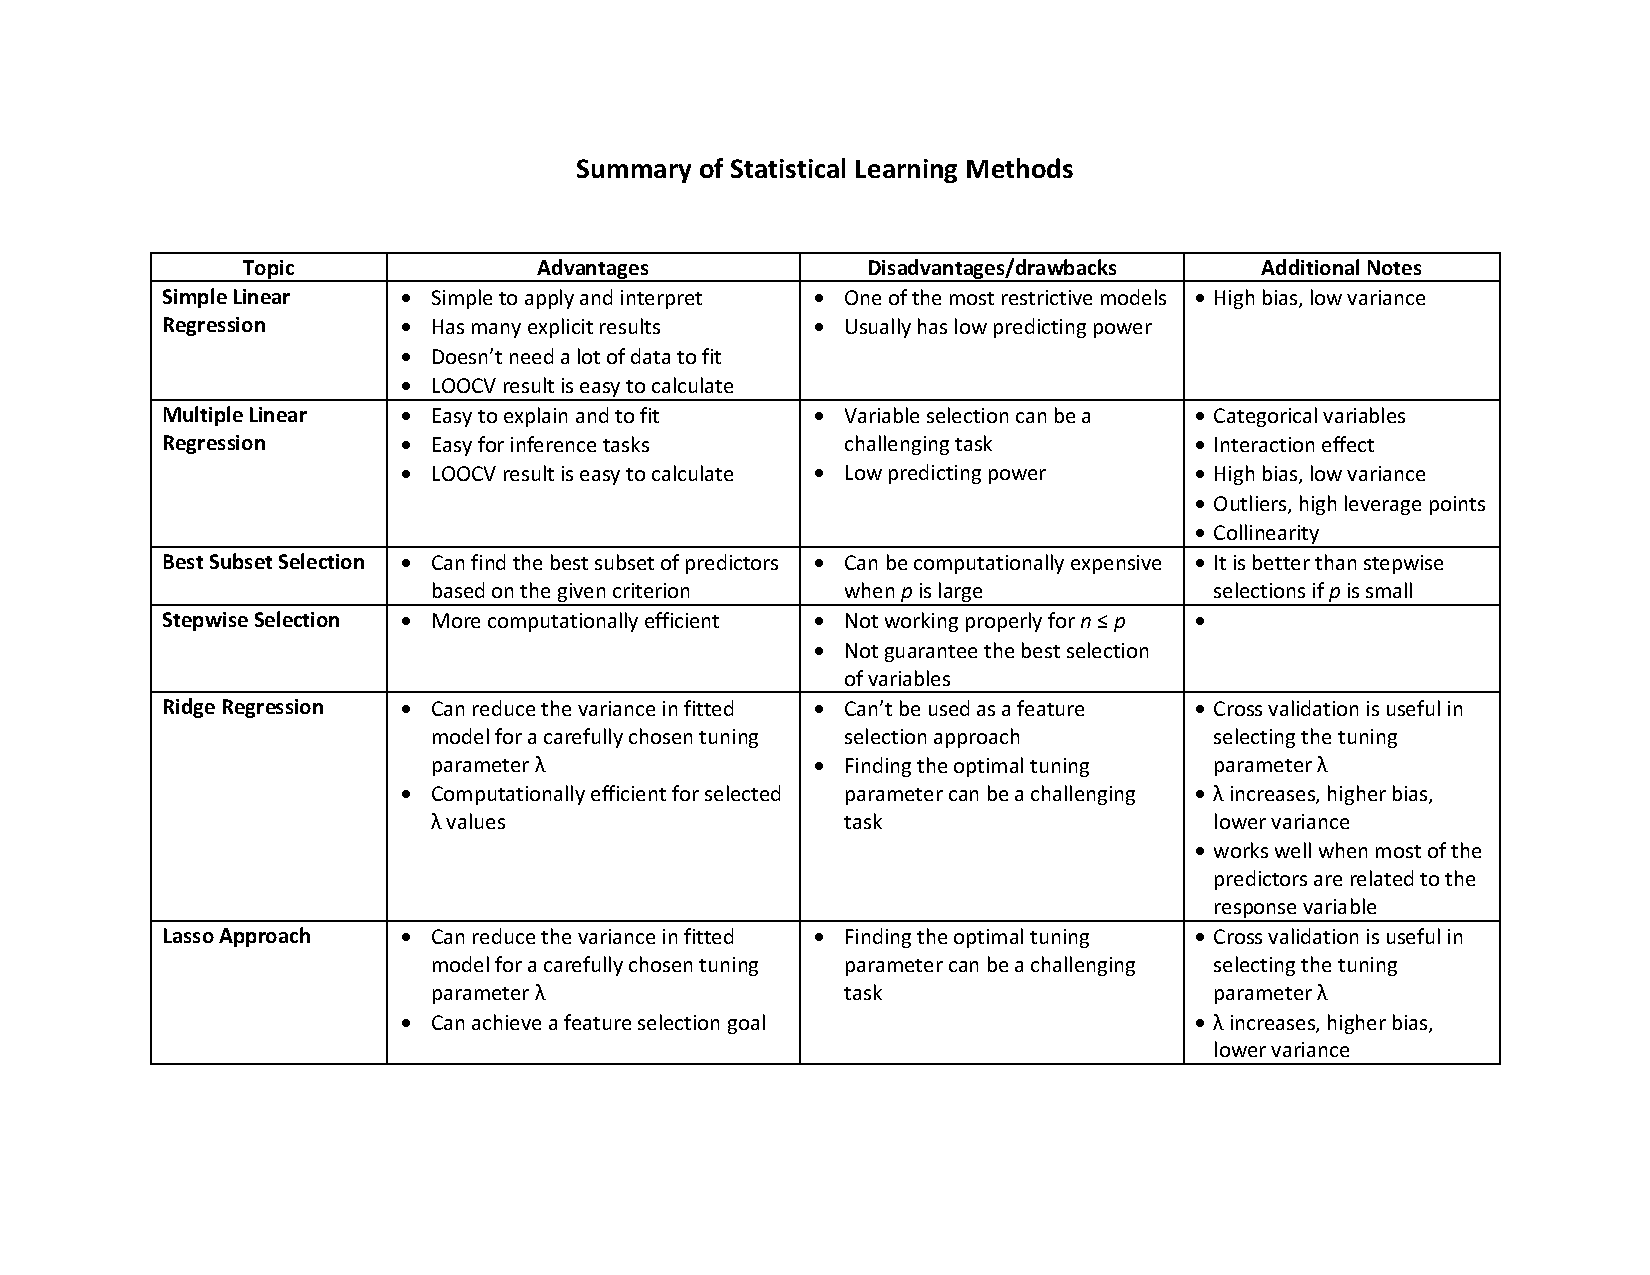
\includepdf[pages=-]{Summary of Statistical Learning Methods_2025.pdf}

\end{document}